% /* spellchecker: disable */
\documentclass[
    12pt,
    a4paper,
    BCOR=10mm,
    %chapterprefix,
    DIV=14,
    listof=totoc,
    bibliography=totoc,
    headsepline
]{scrbook}

% Encoding Options
\usepackage[utf8]{inputenc}
\usepackage[T1]{fontenc}
% Modern latin font
\usepackage{lmodern}
% Language
\usepackage[english]{babel}

% BibLaTex incl. Biber as backend
\usepackage[
    % General options
    backend=biber,
    style=numeric,
    sorting=nyt,
    % Specific options
    % backref=true,
    doi=true,
    eprint=false,
    hyperref=true,
    url=true]{biblatex}
\addbibresource{sources.bib}

% change date format from 'mm/dd/yyyy' to 'dd.mm.yyyy' TODO: revert later?
\renewbibmacro*{url+urldate}{%
\printfield{url}%
\iffieldundef{urlyear}
    {}
    {\setunit*{\addspace}%
    \printtext[urldate]{\printfield{urlday}\setunit*{\adddot\addthinspace}%
            \printfield{urlmonth}\setunit*{\adddot\addthinspace}%
            \printfield{urlyear}%\setunit*{\adddot}
}}}%

\addto\captionsenglish{% Replace "english" with the language you use
    \renewcommand{\contentsname}{Table of Contents}
}

% Load xcolor first
\usepackage[usenames, dvipsnames]{xcolor}

% Various useful packages
\usepackage[footnote]{acronym}
\usepackage{amsfonts}
\usepackage[page]{appendix}
\usepackage{booktabs}
\usepackage{bytefield}
\usepackage{caption}
\usepackage[autostyle,babel,strict]{csquotes}
\usepackage{enumitem}
\usepackage{footnote}
%\usepackage{float}
\usepackage{floatrow}
\usepackage{geometry}
\usepackage{graphicx}
\usepackage{listings}
\usepackage{microtype}
\usepackage{multirow}
\usepackage{pgfplots}
\usepackage[section]{placeins}
\usepackage{scrlayer-scrpage}
\usepackage{subcaption}
\usepackage{tabularx}
\usepackage{textcomp}
\usepackage{tikz}
\usepackage{tikzscale}
\usepackage[titles]{tocloft}
\usepackage{todonotes}
\usepackage{units}
\usepackage{xparse}

\geometry{outer=3.5cm, inner=2.5cm, top=3cm, bottom=3cm}
%\usepackage{showframe}
%\usepackage{layout}

\usetikzlibrary{arrows,calc,patterns,positioning,shapes}
\pgfplotsset{compat=newest}
\usepgfplotslibrary{dateplot, statistics}

% For dates
\newcommand{\leadingzero}[1]{\ifnum #1<10 0\the#1\else\the#1\fi}

% Allow footnotes in tables
\makesavenoteenv{tabular}
\makesavenoteenv{table}

% Use hyperref last to make sure it can define all necessary commands
\usepackage[pdfborder={0 0 0}]{hyperref}

\addto\extrasenglish{%
    \def\chapterautorefname{Chapter}%
    \def\sectionautorefname{Section}%
    \def\subsectionautorefname{\sectionautorefname}%
}
\newcommand*{\Appendixautorefname}{Appendix}

% Floatrow command for tables
\newfloatcommand{capbtabbox}{table}[][\FBwidth]

% Use glossaries/xindy after hyperref to make it use links
\usepackage[acronym,nonumberlist,nopostdot,numberedsection,toc,xindy]{glossaries-extra}
\usepackage[xindy]{imakeidx}

% Command to create dual entries (acronyms with description)
\NewDocumentCommand{\newdualentry}{ m m m m } {%
  \newglossaryentry{gls-#1}{%
      name={#3},%
      description={#4}
  }
  \newglossaryentry{#1}{
      type=\acronymtype,
      name={#2},
      description={#3, \glsseeformat[see:]{gls-#1}{}},
      first={\gls{gls-#1} (#2)\glsadd{gls-#1}}
  }
}

% Setup glossaries
\loadglsentries[main]{misc/glossary}
% \renewcommand*{\glsautoprefix}{ap:gl_}

% Limit ToC depth
% TODO: reenable
\setcounter{tocdepth}{4}
\setcounter{secnumdepth}{4}

% Customize itemize
\setlist[itemize]{itemsep=-0.25em, label=--}

% Page (indent) definitions
\sloppy
\setlength{\parindent}{0em}
\setlength{\parskip}{1.2ex plus 0.5ex minus 0.5ex}

% !TEX root ../thesis
% /* spellchecker: disable */

% ## META ##
\def\title{Reverse Engineering and Monitoring the Dridex Botnet}
\def\author{Florian Wilkens}
\def\email{1wilkens@informatik.uni-hamburg.de}
\def\studentId{6324030}

% ## COLORS ##
\definecolor{light-gray}{gray}{0.85}
\definecolor{comment-green}{HTML}{009900}

\definecolor{lightcyan}{rgb}{0.84,1,1}
\definecolor{lightgreen}{rgb}{0.64,1,0.71}
\definecolor{lightred}{rgb}{1,0.7,0.71}
\definecolor{darkred}{rgb}{0.502,0.082,0.082}

\definecolor{uhhred}{cmyk}{0,100,100,0}

% ## LISTINGS ##
\lstset{
    basicstyle=\ttfamily,
    breakatwhitespace=true,
    breaklines=true,
    captionpos=b,
    commentstyle=\color{comment-green},
    escapeinside={\%*}{*},
    frame=single,
    keywordstyle=\color{blue},
    numbers=left,
    numberstyle=\footnotesize,
    rulecolor=\color{black},
    % prebreak=\textbackslash,
    postbreak=\hbox{\(\hookrightarrow\) },
    showstringspaces=false,
    stringstyle=\color{red},
    tabsize=4
}

\lstdefinestyle{plain}{
    numbers=none
}

\lstdefinestyle{pseudo}{
    morecomment=[l]{//},
    commentstyle=\color{gray},
    keywords={DO, WHILE, IF, NULL, FOR, AND, CONST, GLOBAL},
    keywordstyle=\bfseries
    %numbers=none
}

\lstdefinestyle{asm}{
    language=[x86masm]Assembler,
    keywords={mov, cmp, jnz, xor},
    keywords=[2]{ebx, edx},
    keywordstyle=[2]\color{red},
}

\lstdefinestyle{shell}{
    %language=sh
}

\lstdefinestyle{c}{
    language=C,
    morekeywords={pragma}
}

\lstdefinestyle{win}{
    style=c,
    numbers=none,
    morekeywords={BOOL, FARPROC, HINSTANCE, DWORD, LPVOID}
}

\lstdefinestyle{ida}{
    style=c,
    numbers=none,
    morekeywords={HeapString}
}


% Some pdf related meta-information
\hypersetup{
    pdftitle = {\title},
    pdfauthor = {\author},
    pdfsubject = {Master's Thesis},
    pdfkeywords = {dridex, security, botnet, p2p, reverse engineering}
}

% Define some custom commands for inlining code, file names or shell commands
\newcommand{\mdinline}[1]{\colorbox{light-gray}{\texttt{#1}}}
\newcommand{\shinline}[1]{\textbf{\texttt{#1}}}

% Custom footnote command that adds \hspace before the text
\newcommand{\fnote}[1]{\footnote{\hspace{2pt}#1}}

% Abstract command
\newcommand{\abstract}[1]{\textit{#1}\bigskip}

% Colored bitbox
\newcommand{\colorbitbox}[4][]{%
  \rlap{\bitbox[#1]{#3}{\color{#2}\rule{\width}{\height}}}%
  \bitbox[]{#3}{#4}}

% Tikz commands
\newcommand{\flowarrowclip}[2]{%
    \fill[#2] let \p1 = ($(#1.east arrow tip) - (#1.before east arrow tip)$) in
        (#1.north west) -- ($(#1.north west)!.5!(#1.south west) + (\x1, 0)$) -- (#1.south west) -- ++(-5mm, 0) -- ($(#1.north west) + (-5mm, 0)$) -- cycle;
}
\newcommand{\flowarrowfirst}[4]{%
    \node[arrowbox, fill=#3] (#1) {#2};
    \flowarrowclip{#1}{#4}
}
\newcommand{\flowarrow}[5]{%
    \node[arrowbox, left=of #5.center, fill=#3] (#1) {#2};
    \flowarrowclip{#1}{#4}
}

% Change name of listing from 'Listings' to 'List of Listings' to be consistent
\renewcommand*{\lstlistlistingname}{List of Listings}

\begin{document}

% !TEX root ../thesis
% /* spellchecker: disable */
\newgeometry{centering,left=1.75cm,right=1.75cm,top=3cm,bottom=4cm}
\begin{titlepage}
    \begin{center}
        \noindent\begin{minipage}{0.4\textwidth}% adapt widths of minipages to your needs
            
\includegraphics[width=\linewidth]{img/uhh_logo.pdf}
        \end{minipage}%
        \hfill%
        \begin{minipage}{0.6\textwidth}\raggedright
            Faculty of Mathematics, Informatics und Natural Sciences \\ 
            Department of Informatics \\ 
            Working Group ``Security and Privacy'' \\
            Research Group ``IT-Security and Security Management''
        \end{minipage}

        \vspace*{3cm}

        {\titlefont\huge \title \par}

        \bigskip
        \bigskip

        {\titlefont\Large --- Master's Thesis ---\par}

        %\bigskip
        %\bigskip

        %{\large
        %Research group ``IT Security and Security Management'' \\
        %Working group ``Security and Privacy'' \\
        %\vspace{1em}
        %Department of Informatics \\
        %Faculty of Mathematics, Informatics und Natural Sciences \\
        %University of Hamburg
        %\par}
    \end{center}

    \vfill

    {\large \begin{tabular}{rl}
        Submitted by            : & \author \\
        %E-Mail                  : & \href{mailto:\email}{\email} \\
        Matriculation number    : & \studentId \\
        Course of studies       : & M.Sc. Informatics \\
        \\
        First reviewer          : & Prof.\ Dr.\ Mathias Fischer \\
        Second reviewer         : & Prof.\ Dr.\ Hannes Federrath \\
        Supervisor              : & M.Sc.\ Steffen Haas \\
    \end{tabular}\par}
    \begin{flushright}
        \large Hamburg, \today
    \end{flushright}
\end{titlepage}
\restoregeometry


% !TEX root ../thesis
\chapter*{}

\thispagestyle{empty}

\begin{center}
I would first like to thank Prof. Mathias Fischer for giving me the chance the tackle this interesting challenge. Reverse engineering has always me a dream of mine and I really enjoyed the time spent deciphering Dridex's architecture and protocols.

\bigskip
\bigskip

Additionally, I thank my thesis advisor Steffen Haas for providing invaluable feedback especially in the last days of writing. The discussions with you significantly influenced the shape and content of this thesis.

\bigskip

I am also very grateful to David Jost for his tireless tech support in Python, Latex or Tikz questions. Without you the figures would not be half as pretty.

\bigskip
\bigskip

Finally, I must express my gratitude to my parents and to my girlfriend for providing me with support and continuous encouragement through the process of researching and writing this thesis. This accomplishment would not have been possible without them.
\smallskip

Thank you!
\end{center}

% Nadege?
% David for TEX/TIKZ
% Parents?

\chapter*{Abstract}\label{ch:Abstract}

\thispagestyle{empty}

In the last years \glspl{bn} present a growing threat to end-users and network administrators alike.
The large networks of infected hosts are able to deliver massive \gls{ddos} attacks and allow the \gls{bm} to exfiltrate data from the \glspl{bot} in nearly untraceable ways.
With the evolution from centralized architectures to \gls{p2p} networks \gls{bn} became more resilient to takedown attempts by law enforcement.
As monitoring is more important then ever to evaluate the threats posed by them.
Because of their resilience, exploiting vulnerabilities in communication protocols is often the only way to take down a \gls{bn}.

This thesis analyzes and monitors one of the most dangerous \glspl{bn} today, the Dridex financial trojan, with a focus on its \gls{p2p} protocol.
It provides byte-level descriptions of request and response messages to bootstrap further research.
Addtitionally, details of the sophisticated module execution process as well as the bot main module's internal architecture are presented.
To verify our findings about the \gls{mw} the \emph{Dridex L2 Scanner} was developed, applied to large \gls{ip}-address ranges from Great Britain and Europe and revealed 42 total \glspl{sp} which were then monitored for a short timespan.\\
%
From a protocol standpoint no immediate vulnerabilities could be found in the analyzed messages of Dridex's \gls{p2p} communication besides a minor information leak.
Future research should continue this research to support future takedown attempts.


\microtypesetup{protrusion=false} % disable protrusion locally for the toc
\tableofcontents                  % prints Table of Contents
\microtypesetup{protrusion=true}  % reenable protrusion

% !TEX root ../thesis
\chapter{Introduction\label{ch:Introduction}}

\abstract{In this chapter we describe the motivation and aims of the thesis as well as preview our contributions.
First, we explain why \glspl{bn} pose a threat to the Internet and motivate why \emph{Dridex} should be the focus of research.
Then we briefly summarize the contributions of this thesis and give a general outline of the remaining chapters.}

\section{Motivation\label{sec:Introduction::Motivation}}
\Glspl{bn} are classified as an ever-growing risk to \acrshort{it} security.
A cluster of compromised hosts (\glspl{bot}) is controlled by a \gls{c2} operated by the so-called \gls{bm}~\cite{aburajab2006multifaceted}.
Malicious software (\gls{mw}) is installed on the machines which listens for commands from the \gls{c2} and executes them in the host context.
These \glspl{bot} are then used to perform various malicious actions ranging from spam email delivery and distributed password cracking to full-blown \gls{ddos} attacks using the combined bandwidth available to all available \glspl{bot}.

When the \gls{mw} collects credentials or credit card information from the compromised host it is usually sent back to the \gls{c2}.
While traditional variants send the data directly to the server, \gls{p2p} \glspl{bn} are often organized hierarchically and relay the data to the \gls{c2}.
This helps the \gls{bm} to stay hidden behind multiple layers of interconnected \glspl{bot} and prevent detection by law enforcement.

It is therefore very important to gain insights into the communication protocols used in these sophisticated \glspl{bn} as well as their capabilities in regards to computing power and bandwidth.
This knowledge can then be used to find potential design or implementation flaws in these hugely distributed systems which might aid in global takedown attempts.
As the source code for \glspl{bn} is not freely available and communication with the \gls{c2} is heavily encrypted, the only way to gain insights into the protocols is through reverse engineering the malicious binary samples.
However, \gls{mw} authors often implement a number of techniques to disrupt binary analysis such as obfuscation and packing.
We estimate a significant time will be spent circumventing these protective measures until the relevant parts for message handling can be freely analyzed.

In this thesis, we aim to reverse engineer and analyze one of the most dangerous \gls{p2p} \glspl{bn} today, the Dridex banking trojan.
With over £20 million stolen in the United Kingdom alone (as of 2015), it is one of the most financially damaging trojans~\cite{nca2015uk}.
Often cited for it
Dridex is constantly adapted and updated to remain undetected and the \glspl{bm} behind it are often exploring new alternative revenue streams.
While it started with classical credential stealing, a recent \gls{mw} strain was used to deliver ransomware.
This broadens the target audience from online banking users to potentially every computer user worldwide.


\section{Contributions\label{sec:Introduction::Contributions}}
The reverse engineering process will be largely aided by IDA Pro\fnote{{\url{https://www.hex-rays.com/products/ida/overview.shtml}}}, a professional disassembling tool with advanced reconstruction abilities, as well as other standard tools for debugging, disassembly and other low-level tasks.
This will be essential in understanding the obfuscated binary code of Dridex.
The focus is hereby placed on the communication protocols as they represent the entry point in monitoring the \gls{bn}.
The goal is to provide byte-level descriptions of as many messages as possible which can be used to directly construct valid payloads.
Although the formats of those messages are updated (and hardened) from time to time, the general structure and included information should be useful in bootstrapping further research in the future.
To validate the results obtained from reverse engineering a scanner will be implemented capable of detecting Dridex \glspl{sp} in large \gls{ip}-address ranges.
Finally, the \emph{Dridex L2 Scanner} will then be invoked on some representative subnets to gain some knowledge about the \gls{bn}'s population count.


\section{Outline\label{sec:Introduction::Outline}}
In this first chapter, we highlighted the danger of \glspl{bn}, motivated analysis, takedowns and the Dridex L2 Scanner.
The second chapter summarizes previous research and publications on the topic of \glspl{bn} in general and Dridex in particular.
In \autoref{ch:Reverse_engineering_Dridex} we present the results of the reverse engineering efforts with a special focus on the communication protocols.
In the following chapter, we briefly discuss the scanner's implementation, present our data set of \gls{ip}-address ranges and evaluate the results obtained by the scan.
The final chapter summarizes the work of this thesis and proposes future research based off it.
% !TEX root ../thesis
\chapter{Related work\label{ch:Related_work}}

\abstract{This chapter introduces related work both on \glspl{bn} (especially \gls{p2p} based) in general as well as specifically on Dridex.
Furthermore, it provides a short introduction to the process of reverse engineering and counter-measures to it.}

\section{Botnets\label{sec:Related_work::Botnets}}
\Glspl{bn} can be divided into two major categories based on their architecture: centralized and distributed.
Both types come with tradeoffs regarding ease of development and resilience.

\paragraph*{Centralized architectures}
Simple \glspl{bn} use a single \gls{c2} server to control the infected machines.
Popular choices include \gls{irc} and plain \gls{http} based web servers which expose endpoints for the \glspl{bot} to connect to~\cite{aburajab2006multifaceted}.
The \gls{mw}'s code contains a hardcoded \gls{ip} address (and port) to connect to where the communication backend is hosted.
This architecture trades stability for ease of development and is very vulnerable to takedown attempts.
If the controlling server (or even multiple servers) are taken offline, the \glspl{bot} are no longer a direct threat as no new commands from the \gls{c2} will be received.

To mitigate this single-point-of-failure, multiple approaches exist.
\emph{Mirai}, an \gls{iot} worm used to perform powerful \gls{ddos} attacks, uses domain names instead of hardcoded \gls{ip} addresses to identify its \gls{c2} server.
This enables the \gls{bm} to dynamically switch out the contacted server by modifying the corresponding \acrshort{dns} entry.
Combined with a short \gls{ttl} this solution provides a responsive protection against regular takedown attempts while maintaining relatively low complexity.

However, \gls{dns} based control structures expose other potential weaknesses limiting the \gls{mw} spread.
In 2009 the Spanish based \gls{bn} called \emph{Mariposa} was taken down by \emph{sinkholing} the \gls{c2} domains used to control the \glspl{bot}.
Security operators seized the set of domains in a collaborative effort with domain registrars and law enforcement across several different countries effectively halting all \gls{bn} communication~\cite{krebs2010mariposa, nadji2013beheading}.
To prevent sinkholing, \gls{dns} based \gls{mw} started to transition from hardcoded domain names to \glspl{dga}.
These algorithms include certain environmental factors such as date and time or system language to generate a huge list of potential \gls{c2} domain names.
The \gls{bot} then initiates connections to these domains until one correctly resolves and responds in the correct protocol.
Popular examples such as Conficker-C generated about 50.000 names per day hindering effective sinkholing massively~\cite{porras2009conficker}.
But as the \gls{dga} has to be used in the \gls{mw} it has to be included in the binary and as such can be reverse engineered.
This allows security professionals to predict future results and include the domains in blacklists for example in firewalls or \gls{ids}.

The transition from single hardcoded servers to \gls{dga} based structures increases the robustness of centralized \glspl{bn} massively and makes takedown attempts a lot less likely to succeed completely.
However there are still ways to partially mitigate the impact of \glspl{bn} through netflow analysis and \gls{ids}.


\paragraph*{Distributed architecture}
To avoid \gls{dns} based problems multiple \glspl{bn} have transitioned to \gls{p2p} protocols~\cite{dittrich2008new}.
Instead of a defined \gls{c2} (via \gls{dns} or \gls{dga}) each \gls{bot} now maintains a \emph{\gls{pl}} filled with information about other \glspl{bot} it can connect to.
The \glspl{bm} can issue commands through a selection of special \glspl{bot} which they control directly.
The protocol then ensures these commands are populated and executed throughout the \gls{bn}.
This makes complete disruption of the communication immensely hard as the size of each bot's \gls{pl} can easily reach 1000 and more~\cite{haas2016resilience}.

An important concept in \gls{p2p} networks in general and \gls{p2p} \glspl{bn} especially is the notion of so-called \emph{\glspl{sp}}.
While a regular server is often directly connected to the internet, \glspl{bot} are mostly infected consumer or office machines which are separated from the public address space via firewalls or behind a \gls{nat} device.
This limits their capabilities in the \gls{p2p} network as connections are usually limited to be outbound to other peers, while incoming requests are filtered or blocked.
As connectivity of all \glspl{bot} is the main goal of a \gls{p2p} \gls{bn} it requires some peers to have a publicly routable \gls{ip} address to accept connections from infected hosts behind \gls{nat}.
These \glspl{sp} represent a significantly lower percentage of the total network peers but are invaluable in keeping the network connected.
Rossow et al.\ estimate that only around 13--40\% of the total peers of a \gls{bn} are \glspl{sp}~\cite{rossow2013sok}.
This makes them an ideal target for takedown attempts.


\paragraph*{\gls{p2p} \gls{bn} monitoring}
It is very important to study a \gls{bn} over long periods of time to gain insight about its reach and growth.
Following the evolution from centralized \glspl{bn} to \gls{p2p} networks the security community had to adapt and evolve monitoring techniques.
Since \gls{p2p} \glspl{bn} constantly change when new \glspl{bot} enter or leave the network (this is called \gls{node_churn}), obtained results are quickly outdated or inaccurate.
As a result, monitoring has to be resilient, long-running, and mostly automated to continually gather information.
Main objective is to obtain information about the \emph{full population} (total number of active peers) of a \gls{bn} to estimate its capabilities in regards to computing power and bandwidth.
To achieve this in a \gls{p2p} context, two major approaches exist: \emph{crawling} and \emph{sensor injection}.
\begin{description}
    \item[Crawling]
    A \gls{bn} \gls{crawler} captures data about active \glspl{sp} of the network by continuously requesting the \glspl{pl} of known \glspl{bot} and enumerating them.
    This approach generates a view on the \gls{bn} from the perspective of a regular peer as the online status of non-\glspl{sp} cannot be verified limiting its usefulness in regards to population levels.
    \item[Sensor injection]
    To gain insights from the perspective of a \gls{sp} a \gls{sn} can be injected into the network.
    This node implements the \gls{bn} protocol and acts as fake \gls{sp} similar to a \gls{hp}.
    This approach can be used to verify connections originating from \glspl{bot} behind \gls{nat} and usually produces a more realistic view over the number of active peers.
\end{description}

Unfortunately most major \glspl{bn} employ some method of protection against intelligence gathering and are constantly adapted to limit or block the use of the aforementioned techniques~\cite{rossow2013sok, yan2011ratbot}.


\section{Dridex\label{sec:Related_work::Dridex}}
Dridex is currently one of the most dangerous financial trojans.
Its primary focus is credential theft of online banking sites but it also includes components for remote control of infected machines through \gls{vnc}.
Dridex is the successor of the famous Cridex worm, adding a \gls{p2p} network layer and switching from self-propagation to spam emails as the main distribution vector.
Since its inception in 2014, the \gls{mw} has been constantly updated, to avoid detection by antivirus software and explore new ways to infect targets~\cite{ramos2016dridex, proofpoint2017dridex, teo2015learning, tokazowski2016dridex}.
Internally Dridex is divided into multiple \emph{subnets} which are most likely controlled by different teams with each subnet often focussing on single countries or regions.

While other infection vectors are often explored, spam email campaigns remain the main distribution mechanism of Dridex.
These emails are highly customized targetting a selected country or even a single company and contain malicious attachments often disguised as trustworthy messages such as scanned documents or invoices.
The attached files are mostly Microsoft Office documents or script files with a fake extension which download and launch Dridex.
The user is then tricked into enabling macro execution by a message stating that the document cannot be displayed correctly without them.
Although this behavior is common among phishing emails, Dridex's spam campaigns are of an unusually high quality with very few spelling errors and convincing domain names.
The level of professionalism hints that the organization behind Dridex is highly experienced~\cite{obrien2016dridex}.

\begin{figure}
    \centering
    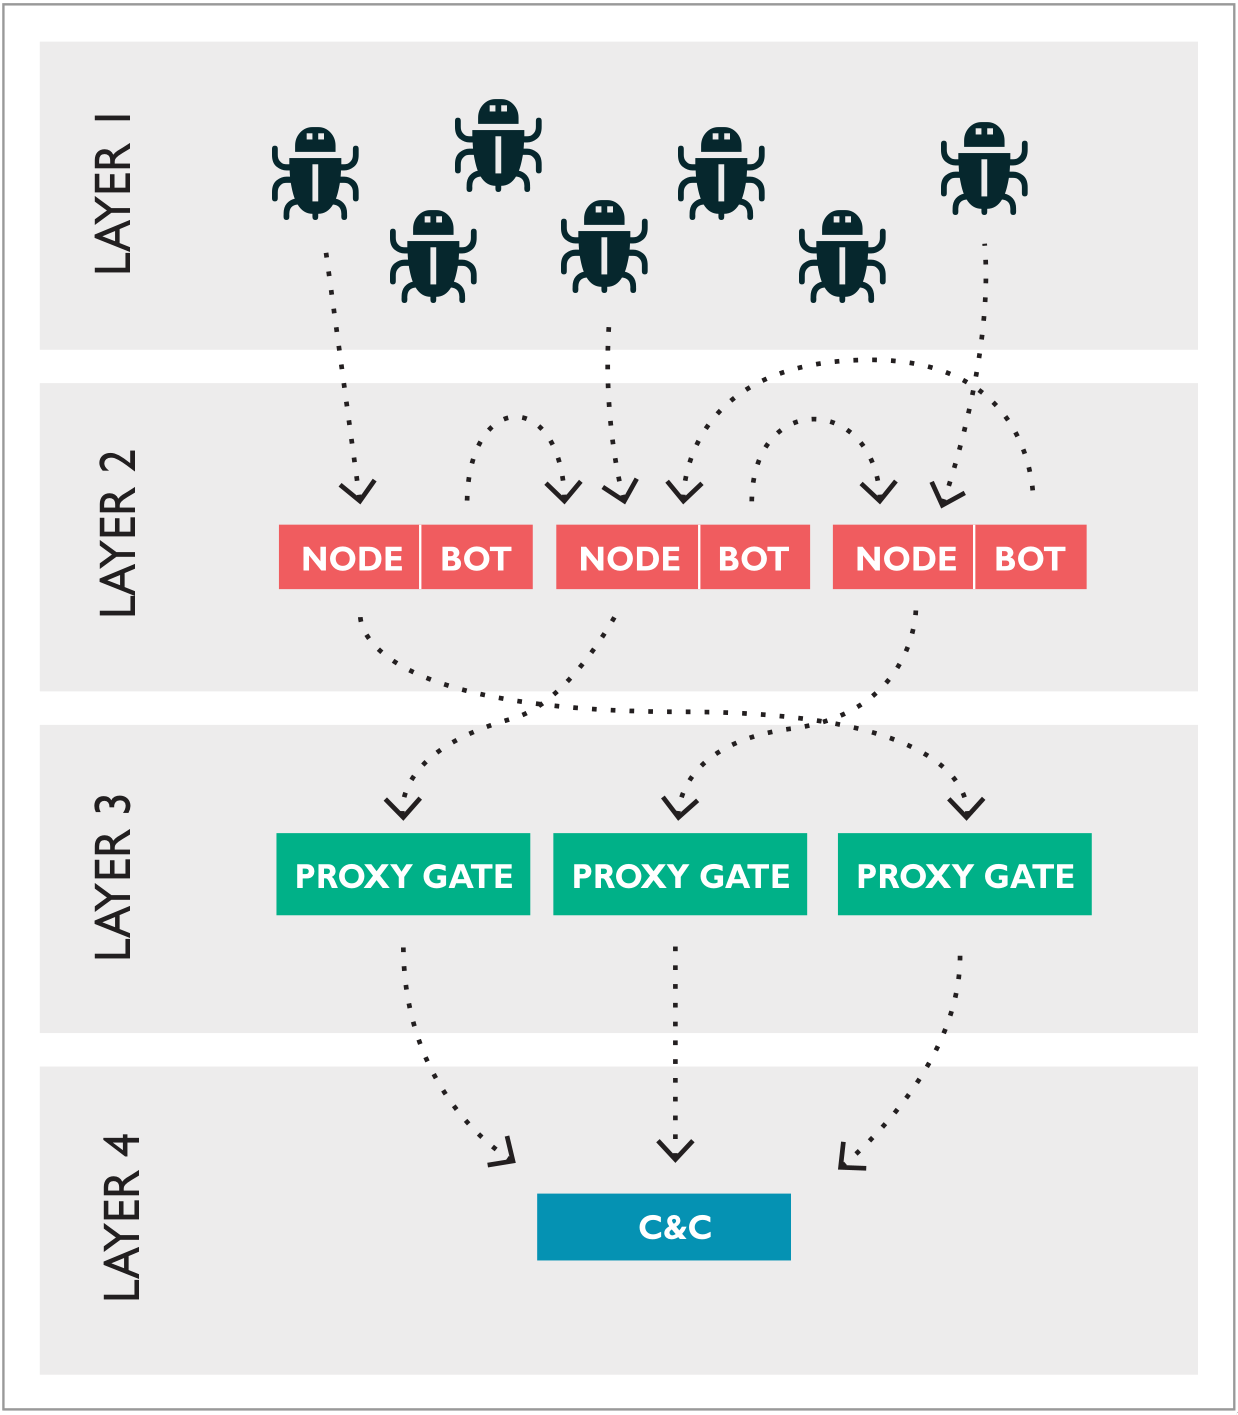
\includegraphics[width=.5\textwidth]{img/dridex_layers}
    \caption[Dridex network layers]{Dridex network layers as described by Blueliv~\cite[Fig. 12]{blueliv2015chasing}\label{fig:Dridex::Network_layers}}
\end{figure}

From a network standpoint, Dridex can be seen as a centralized-\gls{p2p} hybrid \gls{bn}.
It combines \gls{p2p} elements with a strict hierarchy which is atypical for fully decentralized networks.
Additionally, the underlying \gls{p2p} network relies on the hidden \gls{c2} server for orchestration instead of being self-organizing.
As seen in \autoref{fig:Dridex::Network_layers} the \gls{bn} is divided into four main layers starting at the infected machines from layer 1 up to the controlling \gls{c2} server on the fourth layer.
The second layer (L2) is made up of super peers manually elected by the \gls{bm} from the capable \gls{bot} pool, while layer 3 (L3) consists of infected servers which act as proxies to further hide the backend \gls{c2} server~\cite{blueliv2015chasing}.


\section{Reverse engineering\label{sec:Related_work::Reverse_engineering}}
Reverse engineering is a highly iterative process which can be divided into \emph{static} and \emph{dynamic analysis} which are often performed complementary to gain a comprehensive insights on the \gls{mw}'s architecture and behavior.
As the source code is usually not freely available the analyst works with disassembled machine code to reconstruct the high-level behavior.

\begin{description}
    \item[Static analysis] describes the process of tracing the control flow of the assembly code without executing the \gls{mw}.
    The analyst interprets instructions and function calls to determine the purpose of functions or even single blocks.
    This phase often requires significant research on various topics such as operating system \glspl{api}, compiler, and library versions as well as optimizations to decipher the assembly code.
    \item[Dynamic analysis] is performed in a controlled environment where the \gls{mw} gets purposefully executed and monitored.
    This enables the analyst to manipulate execution beyond regular paths by changing register values or skipping instructions.
    Furthermore, resource usage (including network and disk traffic) can be inspected to understand advanced topics such as persistence mechanisms or communication protocols.
\end{description}

Targets of research include communication protocols, membership management, system architecture and general vulnerability analysis.
Successful takedown attempts almost always rely on some sort of weakness in one of these areas~\cite{dittrich2012so}.


\section{Anti-reverse engineering techniques\label{sec:Related_work::Anti_reverse_engineering_techniques}}
As Dridex is a highly successful piece of \gls{mw} we can expect sophisticated obfuscation measures when analyzing the machine code.
The most common technique is \emph{binary packing} which works by applying a mix of compression and encryption to hide the binary from signature based tools.
Yan et al.\ roughly categorize (\gls{mw}) packers in four major categories~\cite{yan2008revealing}.

\begin{description}
    \item[Compressors] are mainly used to reduce file size by applying a regular, off-the-shelf algorithm.
    Although mostly obsolete by modern connection speeds, they are still used today in \gls{mw} and other legitimate use-cases such as archiving and on devices with limited bandwidth.
    Popular compressors are ASPack\fnote{\url{http://www.aspack.com/}} and Ultimate Packer for Executables (UPX)\fnote{\url{https://upx.github.io/}}.
    \item[Crypters] use simple ciphers to prevent the machine code from static analysis.
    As the focus is not on security (the content has to be decrypted eventually anyway) and the \gls{mw} should execute in reasonable time weak algorithms or even simple XORing are commonly chosen.
    \item[Protectors] incorporate techniques from crypters, compressors, and measures to prevent analysis and tampering.
    These include checksums to detect changes in the binary, anti-dumping procedures to hinder direct examination of the malicious code and debugger detection aborting executing in case a debugger is present.
    Besides their use in \gls{mw}, protectors can be found in \gls{drm} applications for instance in the video game industry.
    Themida\fnote{\url{https://www.oreans.com/themida.php}} is a prominent protector.
    \item[Bundlers] produce a single executable containing multiple executable and resource files which unpack themselves in memory only.
    This technique can simplify installation processes and increase usability for the end user.
    Because \gls{mw} often does not require large amounts of raw data besides malicious code they are rarely bundled but regular software (especially targeting non-technical users) may make good use of a bundler.
    An open source example is MoleBox\fnote{\url{https://sudachen.github.io/Molebox/}}.
\end{description}

Breaking packers often involves careful tracking of memory regions (as the decompression/decryption routines are often written to separate allocations first) as well as analysis of the control flow to detect the real entry-point of the \gls{mw}.
After the correct instruction has been reached, execution is stopped, the unpacked executable gets dumped to disk and reloaded into the debugger or disassembler for further analysis.
As packing is often only the first layer of obfuscation the resulting binary may still contain other hurdles such as intentional \emph{dead code}, further \emph{encrypted memory regions} or even complete \emph{virtual machines} which are used to execute the \gls{mw} through custom (or randomized) instruction sets~\cite{you2010malware}.

\section{Summary\label{sec:Related_work::Summary}}
With the recent shift from traditional, centralized \glspl{bn} to \gls{p2p} architectures it becomes even more important to monitor and crawl them to accurately judge the threats they pose.
Dridex is one of the most damaging \glspl{bn} in recent history and has never been openly documented entities making it an ideal target for our research.
The knowledge about its communication protocols and internal architecture could be essential in future takedown attempt.
It is also expected that the \gls{mw} employs several anti-reverse engineering measures which will present a challenge to overcome in the analysis efforts.

% !TEX root ../thesis
\chapter{Reverse engineering Dridex\label{ch:Reverse_engineering_Dridex}}

\abstract{In this chapter we present the results obtained from reverse engineering Dridex.
First an overview of the general infection process is given followed by more detailed descriptions of its different stages.
We then document the observed communication protocols of the loader and main bot modules as closely as possible.
Finally some challenges and obfuscation measure implemented at the various stages of Dridex are briefly discussed.}

All following results were obtained from reverse engineering 32-bit samples of the Dridex loader and main bot module (version 4.24) (hashes are listed in \autoref{ap:Hashes}).
As mentioned in \autoref{sec:Introduction::Contributions} we focus on the communication aspects of the \gls{mw} with the goal to provide packet descriptions of important messages on byte level.
In addition, we explain crucial parts of the \gls{mw} in detail that we can give indications of compromise and to provide helpful insight when Dridex is reverse-engineered on one's own.
The sections describing the communication protocols contain some seemingly trivial figures of message layouts.
This is intentional and should help to recreate these messages byte by byte in future research.

\section{Infection process\label{sec:Reverse_engineering_Dridex::Infection process}}
A regular Dridex infection process consists of multiple stages and includes several technology stacks.
\autoref{fig:Dridex::Infection_process} gives a brief overview of these stages and their resulting artifacts.
First in the \emph{dropper stage} the \emph{loader} binary is retrieved and executed to start the infection.
Afterwards an initial \gls{pl} and the malicious Dridex modules are downloaded from a distribution server.
Finally the host is completely infected and participates in the \gls{bn} while harvesting data from the user in the \emph{bot stage}.
All stages will be explained in greater detail later on in this chapter.

\begin{figure}[htb]
    \centering
    \makebox[\linewidth][c]{
        \begin{tikzpicture}[
            node distance = 0mm and 18mm,
            arrowbox/.style = {arrow box,
                arrow box arrows={east:1cm},
                arrow box shaft width=2.5cm,
                arrow box head extend=0mm,
                line width=0,
                text=white,
                font=\sffamily\bfseries,
                inner sep=5mm,
                minimum height=2.5cm,
                minimum width=10em,
                align=center,
                text width=10em,
            }
        ]
            \flowarrowfirst{S3}{\hspace{2em}\Gls{bot} stage}{BrickRed}{NavyBlue}
            \flowarrow{S2}{\hspace{2em}Loader stage\\\hspace{1.8em}\small{\textcolor{NavyBlue}{(\gls{pl} + \acrshort{dll}s)}}}{Orange}{TealBlue}{S3}
            \flowarrow{S1}{\hspace{2em}Dropper stage\\\hspace{2em}\small{\textcolor{TealBlue}{(loader binary)}}}{Dandelion}{white}{S2}
        \end{tikzpicture}
    }
    \caption{Stages of a typical Dridex infection\label{fig:Dridex::Infection_process}}
\end{figure}

Initial infection is triggered through execution of a generic \gls{mw} \emph{dropper} by the user.
Dridex primarily uses spam emails with malicious attachments for this step for example office documents or intentionally mislabeled script files.
The goal of this stage is to retrieve a loader binary from an infected webserver and save it to disk.
After the binary has been acquired it is silently executed in the background advancing the infection.

Upon execution, the \emph{loader} starts to collect information about the system and contacts a distribution server to download an initial \gls{pl} and malicious modules.
The selection of \acrshort{dll}s downloaded depends on various factors such as system bitness and installed programs.
The communication protocol with the distribution server is detailed in \autoref{subsec:Reverse_engineering_Dridex::Loader_stage::Protocol}.
Finally, the executable modules---especially the main \emph{\gls{bot} module}---are executed via a custom assembly stub.
The execution process including the stub is explained in \autoref{sec:Reverse_engineering_Dridex::Module_execution} while we focus on the bot module's functionality and architecture in \autoref{sec:Reverse_engineering_Dridex::Bot_stage}.

\section{Dropper stage\label{sec:Reverse_engineering_Dridex::Dropper_stage}}
The dropper typically constitutes the first stage in any \gls{mw} infection process.
Its sole purpose is to gain initial code execution on the target machine and bootstrap the infection.
This usually involves either tricking the user into approval for execution or the use of exploits in installed applications.
As mentioned in \autoref{sec:Related_work::Dridex} Dridex almost exclusively relies on malicious email attachments sent out in highly targeted spam campaigns.
These attachments are mostly Microsoft Office documents which prompt the user to enable embedded macros to correctly display the content.
After code execution has been achieved, the real malicious payload is retrieved and executed.
We observed that Dridex mostly uses compromised low-profile websites such as private or inactive blogs and personal webpages as distribution servers for this stage.

The dropper is not the focus of the reverse engineering efforts in the context of this thesis because of the following reasons.
\begin{itemize}
    \item Dridex does not rely on a single, custom dropper but also uses generic \gls{mw} droppers which are already subject of other research.
    \item Droppers in general are usually written in a scripting language and depend only on obfuscation to avoid detection.
    \item Their implementation is not really complex (after de-obfuscation) as they only download and execute the Dridex loader.
    \item The droppers are easily available in the usual \gls{mw} research sources such as VirusTotal\fnote{\url{https://virustotal.com}}.
\end{itemize}

\section{Loader stage\label{sec:Reverse_engineering_Dridex::Loader_stage}}
The loader represents the second stage in a regular Dridex infection process and is responsible for fetching an initial \gls{pl} and the malicious modules as \glspl{dll}.
In contrast to the dropper, it is highly Dridex specific and includes various anti-reverse engineering measures besides the usual code obfuscation which are explained in greater detail in \autoref{sec:Reverse_engineering_Dridex::Obfuscation_measures}.

\subsection{Overview\label{subsec:Reverse_engineering_Dridex::Loader_stage::Overview}}
The loader's execution can be divided into two phases (shown in \autoref{fig:Dridex::Loader::Phases}).
Initially the binary is started by the dropper as a regular process; we call this the \emph{startup phase}.
To avoid detection, this phase quickly starts starts a system binary with regular user permissions to hide itself.
Our sample used \lstinline|svchost.exe| but other common binaries such as \lstinline|spoolsv.exe| and \lstinline|explorer.exe| have also been observed~\cite{bogdan2015dridex, hutchins2017lets}.
After the fake system process is started the loader injects its complete image into the address space and invokes the entry point, starting the \emph{impersonation phase}.
The original loader process then deletes the executing binary and exits, leaving no trace on disk.

\begin{figure}[htb]
    \centering
    \makebox[\linewidth][c]{
        \begin{tikzpicture}[
            node distance = 0mm and 23mm,
            arrowbox/.style = {arrow box,
                arrow box arrows={east:1cm},
                arrow box shaft width=2.5cm,
                arrow box head extend=0mm,
                line width=0,
                text=white,
                font=\sffamily\bfseries,
                inner sep=5mm,
                minimum height=2.5cm,
                minimum width=17.5em,
                align=center,
                text width=15em,
            }
        ]
            \flowarrowfirst{S2}{Impersonation phase\\\small{(inside system binary)}}{BrickRed}{white}
            \flowarrow{S1}{Startup phase\\\small{(started by the dropper)}}{Green}{white}{S2}
        \end{tikzpicture}
    }
    \caption{Phases of the Dridex loader\label{fig:Dridex::Loader::Phases}}
\end{figure}

The newly started impersonation process is easily detectable as it executed under the regular user account instead of the usual \lstinline|NT-AUTHORITY| system account.
This instance of the loader then continues the infection chain and downloads \glspl{pl} and the \gls{bot} modules.
As the same code is used in both phases, the loader has to be able to detect which phase is currently executing.
Our sample performs this detection by comparing the directory of the executing assembly with the constant \lstinline|C:\Windows\system32|.
This check fails in the startup phase as the dropper does not save the binary in the system folder but succeeds in the impersonation phase since the binary which started the process belongs to Windows.

This two-phase behavior complicates reverse engineering the loader because the new fake system process is not immediately debugged when started by the original process.
The analyst first has to find the phase detection branch instruction and manipulate the outcome to achieve execution of the impersonation phase.

\begin{figure}[htb]
    \centering
    \begin{tikzpicture}[thick,node distance=8cm,auto,>=stealth']
        % Define and draw nodes
        \node[] (bot) {\large Infected machine};
        \node[right of=bot] (server) {\large Distribution server};
        \node[below of=bot, node distance=7.5cm] (bot_ground) {};
        \node[below of=server, node distance=7.5cm] (server_ground) {};

        % Draw node lines
        \draw (bot) -- (bot_ground);
        \draw (server) -- (server_ground);

        % Draw lines
        % LOADER STAGE
        \draw[->] ($(bot)!0.2!(bot_ground)$) -- node[above,midway]{Loader request: `list'} ($(server)!0.2!(server_ground)$);
        \draw[<-] ($(bot)!0.3!(bot_ground)$) -- node[below,midway]{\Gls{pl}} ($(server)!0.3!(server_ground)$);

        \draw[->] ($(bot)!0.5!(bot_ground)$) -- node[above,midway]{Loader request: `bot'} ($(server)!0.5!(server_ground)$);
        \draw[<-] ($(bot)!0.6!(bot_ground)$) -- node[below,midway]{Main \gls{bot} binary (\gls{dll})} ($(server)!0.6!(server_ground)$);

        \draw[->, dashed] ($(bot)!0.8!(bot_ground)$) -- node[above,midway]{Loader request: `(d)modX'} ($(server)!0.8!(server_ground)$);
        \draw[<-, dashed] ($(bot)!0.9!(bot_ground)$) -- node[below,midway]{Module binary (\gls{dll})} ($(server)!0.9!(server_ground)$);
    \end{tikzpicture}
    \caption{Communication flow in \texttt{loader} stage\label{fig:Communication::Loader_stage}}
\end{figure}

The communication flow of the loader stage is shown in \autoref{fig:Communication::Loader_stage}.
First the loader connects to a distribution server and retrieves an initial \gls{pl} consisting of layer 2 nodes for the Dridex subnet (cf:~\autoref{sec:Related_work::Dridex}).
These servers are usually webservers which have been hacked and repurposed by the Dridex operators to act as a \gls{cdn} for their malware.
It seems that the data served by the distribution servers is static without any connections to the backend of the \gls{bn}.
This theory is also supported by the comparatively weak encryption scheme of the communication protocol in this stage (cf:~\autoref{subsec:Reverse_engineering_Dridex::Loader_stage::Protocol}).
After the \gls{pl} has been downloaded, the loader proceeds to retrieve various modules including the main \gls{bot} module.
The selection of modules to be requested depends on the system configuration and some other unknown factors.
Although the server responses contain fully valid Windows \glspl{dll} including \gls{pe} headers the modules are not written to disk but instead kept in memory for later use.
Finally, the executable modules are started as described in \autoref{sec:Reverse_engineering_Dridex::Module_execution} concluding the loader stage.

\subsection{Protocol\label{subsec:Reverse_engineering_Dridex::Loader_stage::Protocol}}
The loader uses an encrypted binary protocol to request the \gls{pl} and modules from the distribution server.
Each message in the \emph{loader protocol} is encrypted with an RC4 key, wrapped in an \emph{envelope} and send to the server via an \gls{http}/\gls{https} \lstinline|POST| request.
The layout of this envelope is detailed in \autoref{bf:Loader::Envelope}.

\begin{quote}
\textbf{Remark:} We use \(\langle~\cdots~\rangle\) in protocol descriptions to indicate content with variable length.
Furthermore, multibyte integers are always assumed to be in \emph{network byteorder} (big endian) if not specified otherwise.
\end{quote}

The first 4 bytes are occupied by the CRC32 checksum of the encrypted message and are followed by the message itself.
The RC4 key used to encrypt the message is hard-coded in the binary\fnote{the analyzed sample used \lstinline|lFAbIz6gtBgS33hffqhdGCdMTgSeBj1BUAB3AuYQG91a0Tq1JhyF7z| \lstinline|LEmMJcQyE42QOqUSPMdaXpsvF1p95YabYpPdHOFG|} and likely changes throughout multiple Dridex campaigns/subnets.
Altough the encryption scheme of the loader protocol is not very sophisticated it makes sense to use RC4 in combination with as static key.
At this point the host is not yet infected and the primary objective is to download and execute the malicious payload.
Cleartext communication is easily detectable by an \gls{ids} once the protocol is deciphered, while a more complicated algorithm like RSA requires more setup on the distribution server and introduces overhead which might slow down the infection.
As the loader is invoked early in the infection process it is often quickly available in \gls{mw} databases which would potentially leaks the encryption key which would require new RSA keys for each campaign.
RC4 keys can be created much easier than RSA and provide a decent middleground between security and flexibility.

\begin{figure}
    \centering
    \begin{bytefield}[bitwidth=\linewidth/10]{8}
        \bitheader{0-7} \\
        \bitbox{4}{CRC32} & \bitbox[rt]{4}{} \\
        \wordbox[blr]{2}{(RC4) Encrypted message\\\(\langle~\cdots~\rangle\)} \\
    \end{bytefield}
    \caption{Loader protocol: envelope layout\label{bf:Loader::Envelope}}
\end{figure}

The \emph{request message} contained in the envelope also follows a specific format after decryption.
\autoref{bf:Loader::Request} shows the layout of a request message in the loader protocol.
Each request contains some information identifying the system as well as a 4 byte integer to signal which content the loader is requesting from the distribution server.
This \emph{message type} is is the only dynamic value of the message while the other fields are required for the distribution server to return the correct payload.
The first piece of information is the host's \emph{BotId}; a value which is contains the computer name and a hash of various constant system properties such as install time and user account name.
This string essentially fingerprints the system and is crucial in monitoring Dridex as assigned \gls{ip} addresses might change in between population snapshots.
Interestingly it also directly contains the computer name in cleartext, which might be helpful when trying to reach out to the user of infected systems.
The BotId is encoded by a 1 byte integer indicating the length of the string followed by the raw \gls{ascii} characters.
This string encoding---with length fields up to 4 bytes---is commonly used throughout all Dridex protocols in places where the data to transmit has a variable length or could contain null bytes.
The next 20 bytes consist of an unknown string value computed from the result of the \gls{api} call \lstinline|GetVolumeInformation| which could not be fully reverse engineered.
The message continues with 2 bytes which are most probably used to indicate the \emph{subnet} or \emph{campaign Id} to the distribution server (cf:~\autoref{sec:Related_work::Dridex}).
This theory could also not be fully verified but both the length and position of the value heavily suggest that the field is used in that way.
The \emph{system configuration} takes up the next 4 bytes.
It is a combination of various security settings and version numbers of the Windows instance running on the host.
The following 4 bytes are occupied by the aforementioned message type which is essentially just the CRC32 checksum of a string indicating the type of the content requested.
An overview of the available message types as well as some related information can be found in \autoref{tab:Loader::Message_types}.
The last byte in the message indicates the system's bitness as a regular number (\lstinline|0x40/64 = 64-bit|).
This is highly important information for the distribution server, as Dridex is distributed in both 32-bit and 64-bit binaries.

\begin{figure}
    \centering
    \begin{bytefield}[bitwidth=\linewidth/10]{8}
        \bitheader{0-7} \\
        \bitbox{1}{\let\bw=\width\ \vspace{.5em}\resizebox{\bw}{!}{\,Length\,}} & \bitbox[rt]{7}{} \\
        \wordbox[lr]{3}{\vspace{-1em}\textbf{BotId}\\\(\langle~\cdots~\rangle\)} \\
        \bitbox[lb]{2}{} & \bitbox[trl]{6}{} \\
        \wordbox[lr]{1}{Unknown 20 byte string} \\
        \bitbox[lr]{6}{} & \bitbox[trl]{2}{\let\bw=\width\ \vspace{.5em}\resizebox{\bw}{!}{\,Possibly \textbf{subnet Id}\,}} \\
        \bitbox{4}{System configuration} & \bitbox{4}{\textbf{message type}} \\
        \bitbox[rlb]{1}{\let\bw=\width\ \vspace{.5em}\resizebox{\bw}{!}{\,\acrshort{os} bitness\,}} \\
    \end{bytefield}
    \caption{Loader protocol: request message layout\label{bf:Loader::Request}}
\end{figure}

Additionally, the first request sent to the distribution server contains extended information about the system such as a list of \emph{installed programs}, the \emph{command line} the loader was executed with and the defined \emph{environment variables}.
This data is only collected in newer versions of Dridex and helps the \glspl{bm} to block security analysts by detecting common research \glspl{vm} or execution in commercial \glspl{sandbox}.
Based on this information the distribution server can blacklist the associated \gls{ip} address and prevent the analyst from obtaining samples of the modules in the first place~\cite{griffin2016dridex}.
Each piece of information is saved in a single string which is encoded in the request as an integer describing the length followed by the character bytes.
All three strings are then directly appended to the message following the layout described in \autoref{bf:Loader::Request}.

\begin{description}
    \item[Installed programs] The list of installed programs is read from the registry key \footnotesize{\lstinline|HKEY_LOCAL_MACHINE\SOFTWARE\Microsoft\Windows\CurrentVersion\Uninstall|}.
    The loader then queries each entry for the subkeys \lstinline|DisplayName| and \lstinline|DisplayVersion|.
    These values are formatted in the following way and finally concatenated.

    \mdinline{<DisplayName> (<DisplayVersion>);}
    \item[Command line] The command line is retrieved via the Windows \gls{api} function \lstinline|GetCommandLineW| and then appended to a constant prefix which is stored encrypted in the binary.

    \mdinline{Starting path: <command line>;}
    \item[Environment] The environment variables are also retrieved from the Windows \gls{api} by calling \lstinline|GetEnvironmentStrings|.
    Each result is formatted in a basic key-value style and concatenated to a single string.

    \mdinline{<name>=<value>;}
\end{description}

As shown in \autoref{fig:Communication::Loader_stage} the loader first downloads an initial layer 2 \gls{pl} follwed by multiple modules (including the main bot module).
Some modules are always downloaded while others are only requested when the system fulfills certain requirements.
These supplementary modules provide extra functionality that is not included in the main bot binary.
All message types (and their corresponding payloads) found in our loader sample are shown in \autoref{tab:Loader::Message_types}.
While we focussed on the main bot module, two other modules are also executable.
\lstinline|mod9| is commonly known as an anti-virus killer module and is only requested when a TrendMicro anti-virus solution is installed on the host while the purpose of \lstinline|mod10| is unknown
The other modules provide functionality like privilege escalation (\lstinline|mod5|), \gls{vnc} remote control and spamming~\cite{wayne2016whats, obrien2016dridex}.
For completeness, we also include whether a payload was always requested in our sample although no further research on the exact conditions was performed.

\begin{table}
    \centering
    \makebox[\linewidth][c]{
        \begin{tabular}{rlrl}
            \toprule
            % Header
            Payload &
            Message Type &
            Executable &
            Always requested? \\
            \midrule

            % 'list'
            \texttt{list} &
            \texttt{0x44C8F818} &
            no &
            yes\\

            % 'bot'
            \texttt{bot} &
            \texttt{0x011F0411} &
            yes &
            yes\\

            % 'mod9'
            \texttt{mod9} &
            \texttt{0xF5175A74} &
            yes &
            no\\

            % 'mod10'
            \texttt{mod10} &
            \texttt{0x6B9FF756} &
            yes &
            yes\\

            % 'dmod7'
            \texttt{dmod7} &
            \texttt{0x997B8EFF} &
            no &
            yes\(^\dag\)\\

            % 'dmod8'
            \texttt{dmod8} &
            \texttt{0x09C4936E} &
            no &
            yes\(^\dag\)\\

            % 'dmod9'
            \texttt{dmod9} &
            \texttt{0x7EC3A3F8} &
            no &
            yes\(^\dag\)\\

            % 'dmod5'
            \texttt{dmod5} &
            \texttt{0x7775EFD3} &
            no &
            yes\\

            % 'dmod6'
            \texttt{dmod6} &
            \texttt{0xEE7CBE69} &
            no &
            yes\\
            \bottomrule
            \multicolumn{4}{l}{\(^\dag\) one of these modules is always requested} \\
        \end{tabular}
    }
    \caption{Loader protocol: message types \& payloads\label{tab:Loader::Message_types}}
\end{table}

At this point the loader has now downloaded the \gls{pl} and all modules according to the system configuration.
In the following we explain how the executable ones are launched on the host, continueing the infection process.

\begin{quote}
\textbf{Remark:}
Due to the very short uptime of the distribution servers as well as time constraints we were not able to successfully download a main bot binary and \gls{pl} directly.
Instead a \gls{dll} was retrieved from VirusTotal\fnote{\url{https://virustotal.com}} and an execution stub was custom built based off information from loader and bot module.
\end{quote}


\section{Module execution\label{sec:Reverse_engineering_Dridex::Module_execution}}
All modules retrieved by the Dridex loader are regular Windows \gls{pe} \glspl{dll} and as such not directly executable.
To perform their malicious purpose they have to be executed inside loader process created earlier and injected into all processes which might handle sensitive user data (e.g.\ web browsers or email clients).

Before we explain how Dridex executes its modules, we recap how \glspl{dll} are supposed to be loaded in Windows.
Normally a program calls the Windows \gls{api} functions \lstinline|LoadLibrary| or \lstinline|LoadLibraryEx|, located in \lstinline|kernel32.dll|, and provides the file name.
These functions load the library's dependencies from the \emph{Import Table}, perform some setup work like base relocation and finally call the library's entry point function: \lstinline|DllMain|.
\autoref{lst:Signature::DllMain_Windows} shows the mandatory signature of this function according to Microsoft.
If a library is loaded through \lstinline|LoadLibrary|, \lstinline|fdwReason| is set to \lstinline|DLL_PROCESS_ATTACH| and \lstinline|lpvReserved| is set to \lstinline|null| indicating a dynamic load\fnote{For further documentation see:~\url{https://msdn.microsoft.com/en-us/library/windows/desktop/ms682583(v=vs.85).aspx}}.

\begin{lstlisting}[style=win, caption={Signature of \texttt{DllMain} according to Microsoft}, label={lst:Signature::DllMain_Windows}]
BOOL __stdcall DllMain(
  _In_ HINSTANCE hinstDLL,    // base address of the DLL
  _In_ DWORD     fdwReason,   // call reason
  _In_ LPVOID    lpvReserved) // indicates load type)
\end{lstlisting}

However, \lstinline|LoadLibrary| and \lstinline|LoadLibraryEx| are often monitored by \glspl{sandbox} and antivirus software as \gls{mw} often loads itself in the process as a library.
In addition, they only work with file names which means the library has to be persisted on disk (or at least on a file system).
To avoid detection and disk-writes, the Dridex loader does not call these functions and instead includes an assembly stub to load a module into memory which is stored encrypted and hex-encoded in the \lstinline|.rdata| section of the binary.
This stub is present in both 32 and 64 bit and includes a custom implementation of \lstinline|LoadLibrary|.
The tweaked function also performs the regular setup work but calls \lstinline|DllMain| slightly differently. 
\autoref{lst:Signature::DllMain_Dridex} shows the modified signature; instead of the \lstinline|lpvReserved| parameter a pointer to an initialization \lstinline|struct| is passed.
While the struct is verified and used in \lstinline|DllMain| the analyzed sample included a fallback routine which was triggered in case an invalid pointer is passed.
This routine would then allocate a new instance of the initialization \lstinline|struct|, prepare it and call \lstinline|DllMain|.
This function is also called if the \gls{mw} is started after a reboot.
Dridex's persistence mechanism keeps the module binaries in memory and only saves them to disk on shutdown alongside a registry entry to relaunch itself on the next boot via \lstinline|rundll32.exe|~\cite{bogdan2015dridex}.
In this case no initialization struct is passed and Dridex has to rely on the fallback routine for successful execution.
\\

\begin{lstlisting}[style=win, caption={Signature of \texttt{DllMain} in Dridex modules}, label={lst:Signature::DllMain_Dridex}]
BOOL __stdcall DllMain(
  _In_ HINSTANCE         hinstDLL,    // base address
  _In_ DWORD             fdwReason,   // call reason
  _In_ DridexInitStruct *initStruct
)
\end{lstlisting}

The execution flow of a module is shown in \autoref{fig:Flow::ModuleExecution}.
First the loader process decrypts the assembly stub embedded in the binary and places it in a buffer.
Next it allocates and prepares an instance of the initialization struct \lstinline|DridexInitStruct| in its own address space and attaches it to the same buffer which is then injected into the foreign process via Atom Bombing (cf:~\autoref{subsec:Reverse_engineering_Dridex::Obfuscation_measures::Atom_Bombing}).
To continue the loader invokes the stub via the internal Windows \gls{api} \lstinline|NtQueueAPcThread|.
The stub---now in the foreign process---passes control to the module's entry-point with the aforementioned signature and passes the initialization struct instance as the third argument.

\begin{figure}
    \begin{tikzpicture}
        \begin{scope}
            \node[anchor=south west] at (0, 0) {\large Loader process};
            \draw[dashed] (0, 0) rectangle (5,-7);

            \fill[fill=red!70] (0.5, -0.5) rectangle (3.5,-4);

            \fill[fill=blue!60] (0.5, -4.5) rectangle (3.5,-6.5);

            \fill[fill=green!50] (2, -5) rectangle (3.25,-6.25);
        \end{scope}

        \begin{scope}[xshift=6.9cm]
            \node[anchor=south west] at (0, 0) {\large Injected process};
            \draw[dashed] (0, 0) rectangle (5,-7);
    
            \fill[fill=red!30] (0.5, -0.5) rectangle (3.5,-4);
    
            \fill[fill=blue!30] (0.5, -4.5) rectangle (3.5,-6.5);
            \fill[fill=green!30] (2, -5) rectangle (3.25,-6.25);
        \end{scope}

        \draw[->,>=latex,line width=1.25pt] (3.8, -3) -- node[above,pos=0.475]{Phase 1: Inject} (7.25, -3);
        \draw[<-,>=latex,line width=1.25pt] (9.75, -1.75) -- (11, -1.75) -- node[above,midway,sloped]{Phase 2: Execute module} (11, -5.75) -- (9.75, -5.75);

        \node[fill=red!70,anchor=east] (A) at (0.5, -7.5) {};
        \node[anchor=west,right=1.5ex] at (A) {Dridex module};
        
        \node[fill=blue!60,anchor=east] (A) at (5, -7.5) {};
        \node[anchor=west,right=1.5ex] at (A) {Assembly stub};

        \node[fill=green!60,anchor=east] (A) at (9, -7.5) {};
        \node[anchor=west,right=1.5ex] at (A) {DridexInitStruct};
    \end{tikzpicture}
    \caption{Module execution via assembly stub\label{fig:Flow::ModuleExecution}}
\end{figure}

\lstinline|DridexInitStruct| contains various information to control the execution of the module as well as addresses of various Windows \gls{api} functions used by the stub itself.
\autoref{tab:Struct::DridexInitStruct} highlights the most important fields of \lstinline|DridexInitStruct|.
The fields \lstinline|stubBaseAddress|, \lstinline|WinApiNames|, \lstinline|sizeModule| and \lstinline|ptrModule| are used by the stub during the custom \lstinline|LoadLibrary| implementation while \lstinline|threadId|, \lstinline|hModuleThread| and \lstinline|stubLoopCondition| can be manipulated by the module itself to manage control flow in the stub.

\begin{quote}
\textbf{Note:} As the byte layout for this struct is extremely important in bootstrapping module execution its complete definition can be found in the \autoref{lst:Types::DridexInitStruct_full}.
\end{quote}

\begin{table}[htb]
    \centering
    \makebox[\linewidth][c]{
        \begin{tabular}{rcrl}
            \toprule
            Offset  &
            Size    &
            Name    &
            Description \\
            \midrule

            \texttt{0x0000} &
            \texttt{0x04}   &
            stubBaseAddress &
            Base address of the stub \\

            \texttt{0x0004} &
            \texttt{0x04}   &
            magicNumber     &
            Must match \texttt{0x56473829} \\

            \texttt{0x0008} &
            \texttt{0xF4}   &
            winApiNames     &
            Names of various important Windows \glspl{api} \\

            \multicolumn{2}{c}{\vdots} & \multicolumn{2}{c}{\vdots} \\

            \texttt{0x0128} &
            \texttt{0x04}   &
            threadId        &
            Id of the Thread to launch \\

            \texttt{0x012C} &
            \texttt{0x04}   &
            sizeModule      &
            Size of the module \\

            \texttt{0x0130} &
            \texttt{0x04}   &
            ptrModule       &
            Pointer to the module allocation \\

            \texttt{0x0134} &
            \texttt{0x04}   &
            hModuleThread   &
            Handle of the started child thread \\

            \texttt{0x0138}   &
            \texttt{0x04}     &
            stubLoopCondition &
            Condition of the stub main loop \\

            \multicolumn{2}{c}{\vdots} & \multicolumn{2}{c}{\vdots} \\

            \bottomrule
        \end{tabular}
    }
    \caption{Important fields of \lstinline|DridexInitStruct|\label{tab:Struct::DridexInitStruct}}
\end{table}

As calling \lstinline|DllMain| blocks the executing thread, the module starts a sub thread to carry out the desired task and saves a handle to it in \lstinline|DridexInitStruct.hModuleThread|.
Hereby the field \lstinline|DridexInitStruct.threadId| instructs the module which functionality should be executed.
The loader always initializes this field with 0 but the module can change it to schedule itself to be re executed with a different value.
The stub then waits on the module thread via the usual Windows \gls{api} function \lstinline|WaitForSingleObject|.
After the thread exits, the module is unloaded and the stub checks \lstinline|DridexInitStruct.stubLoopCondition| whether the module should be reloaded.
This mechanism permits a module to re-execute itself multiple times inside the same process.
\autoref{lst:Pseudo::Stub_ExecuteModule} shows this main loop of the assembly stub in pseudo code.
\\

\begin{lstlisting}[style=pseudo, caption={Module execution loop in assembler stub}, label={lst:Pseudo::Stub_ExecuteModule}]
// Stub_ExecuteModule(DridexInitStruct)
// Continuously execute a module by loading and freeing
%*\textbf{Stub\_ExecuteModule(\rmfamily\textit{i})}*
    ModuleSetup(%*\rmfamily\textit{i}*)
    DO
        LoadLibraryCustom(%*\rmfamily\textit{i}*, %*\rmfamily\textit{i.ptrPayload}*)
        WaitForSingleObject(%*\rmfamily\textit{i.hModuleThread}*, %*\rmfamily\textit{INFINITE}*)
        FreeLibraryCustom(%*\rmfamily\textit{i}*, %*\rmfamily\textit{i.ptrPayload}*)
    WHILE (%*\rmfamily\textit{i.stubLoopCondition}* %*\(\neq\)* 0)
    ModuleTearDown(%*\rmfamily\textit{i}*)
\end{lstlisting}

\vspace{1em}
So far, we described the first two stages in a Dridex infection as well as the module execution across user processes.
The next section contains our findings about the main bot module responsible for \gls{bn} communication as well as data exfiltration to the \gls{c2} as well as detailed protocol description on byte-level.

\section{\Gls{bot} stage\label{sec:Reverse_engineering_Dridex::Bot_stage}}
The \gls{bot} stage is entered after the loader executes the main \gls{bot} module via the assembler stub.
This stage pursues two main goals: Establish a connection to the \gls{bn} and register a new infected host as well as prepare the machine to steal data and credentials.

\subsection{Overview\label{subsec:Reverse_engineering_Dridex::Bot_stage::Overview}}
The main \gls{bot} module is structured into multiple threads with distinct functionalities.
While each main thread can and often does start other helper threads to perform background work, generally only one of the main threads is active at a time.
The \lstinline|DllMain| of the main \gls{bot} module performs some checks, on the filename of the executable in particular, verifies \lstinline|DridexInitStruct.magicNumber| and then launches a thread based on the value in \lstinline|DridexInitStruct.threadId|.
The possible values are described below as well as the corresponding functionality.

\begin{table}[htb]
    \centering
    \begin{tabular}{rl}
        \toprule
        \lstinline|threadId| &
        Functionality\\
        \midrule

        0 &
        Startup \& Initialization\\

        1 &
        \Gls{bn} communication\\

        2 &
        Browser hooking (Internet Explorer, Firefox \& Chrome)\\

        %2.2 &
        %Browser hooking (Google Chrome) \\

        %2.3 &
        %Browser hooking (Mozilla Firefox) \\

        3, 5 &
        Application hooking (via \lstinline|TranslateMessage| \& \lstinline|GetClipboardData|)\\

        4 &
        Synchronization logic\\

        6 &
        Generic Windows \gls{api} hooking of \lstinline|MessageBoxIndirectW|\\
        \bottomrule
    \end{tabular}
    \caption{Main \gls{bot} module threads\label{tab:Main_module::Threads}}
\end{table}

\begin{description}
    \item[Startup \& Initialization] This is the initial thread started by the launcher through the assembly stub.
    It enumerates the user processes and injects each suitable one with the module and an appropriate \lstinline|threadId|.
    One factor for the decision which id is selected, is the CRC32 of the executable name used to detect browser processes.
    The value gets computed for the process to inject and compared with a set of known constants for common browsers (shown in \autoref{tab:Main_module::BrowserCRC32}).
    If a match is found, the process is selected for \lstinline|threadId| \textbf{2} and injected.
    Further details about this decision process as well as the exact injection routines were out of scope of this thesis.
    \item[\Gls{bn} communication] The second thread is responsible for the complete \gls{bn} communication.
    When the initialization thread is finished it re-executes itself through the assembly stub with id \textbf{1} (cf:~\autoref{lst:Pseudo::Stub_ExecuteModule}) inside the supervision process.
    It starts multiple threads in the background to handle the different communication protocols and register itself to the \gls{c2}.
    One sub-thread in particular opens, binds, and listens on a socket accepting the \emph{\gls{p2p} protocol} used between bot and L2 node.
    We observed that the handler function for this socket is able to respond to a certain message which is only send to L2 nodes.
    This indicates that the node functionality is embedded into the main bot module and the bot is effectively able to act as a L2 node without being instructed by the \gls{c2}.
    \item[Browser hooking] This thread is responsible for hooking browser \glspl{api}.
    It hooks the relevant functions for the specific browser to intercept requests and responses to steal credentials according to the configuration.
    It can therefore be seen as the most important thread in regards to data collection on the infected machine.
    Details of the internal data structures storing the gathered data as well as the actual hooks were not part of the conducted analysis.
    \item[Application hooking] Threads \textbf{3} and \textbf{5} hook \lstinline|TranslateMessage| and \lstinline|GetClipboardData| and contain code to take screenshots to harvest data from the user.
    It remains unclear what condition triggers injection of these \lstinline|threadId|s as well as the exact differences between them.
    \item[Synchronization logic] The thread with id \textbf{4} seems to be responsible for synchronization between the multiple components.
    It uses \lstinline|WaitForMultipleObjects| and \lstinline|ReleaseMutex| on certain named synchronization primitives to ensure proper resource management.
    As this functionality was more related to the internal workings of Dridex it was not further analyzed.
    \item[Generic Windows \gls{api} hooking] The last thread seems to be tailored to programs using the Windows \gls{api} \lstinline|MessageBoxIndirectW| to collect sensitive information from the user.
    It hooks this function to collect and store this information for later exfiltration to the \gls{c2}.
\end{description}

\begin{table}
    \centering
    \begin{tabular}{rcl}
        \toprule
        Executable name &
        CRC32 &
        Browser \\
        \midrule

        ``firefox.exe'' &
        \texttt{0xB4E35F10} &
        Mozilla Firefox \\

        ``iexplore.exe''  &
        \texttt{0xC3DDC6D5} &
        Microsoft Internet Explorer \\

        ``chrome.exe'' &
        \texttt{0x9C1D0D0E} &
        Google Chrome \\
        \bottomrule
    \end{tabular}
    \caption[CRC32 of browser executables]{CRC32 of browser executables Dridex is able to hook\label{tab:Main_module::BrowserCRC32}}
\end{table}

\subsection{Protocols\label{subsec:Reverse_engineering_Dridex::Bot_stage::Protocols}}
The main bot module uses multiple protocols to communicate with differend endpoints.
The communication with the \gls{bm} is performed through the \emph{\gls{c2} protocol} while messages messages between bots and L2 nodes rely on the \emph{\gls{p2p} protocol}.

\begin{description}
    \item[\gls{c2} protocol] This protocol is mainly used for data exfiltration or confirmation of \gls{sp} elevation of new \glspl{bot}.
    Messages are encrypted with the \gls{c2}'s public key which is embedded in the main \gls{bot} module itself and signed with a generated RSA private key that is transmitted to the \gls{c2} as part of the registration process.
    As this protocol is more complex and not tremendously useful in determining whether a host is infected, it is not focus of this thesis.
    However it should be studied in future research to potentially be able to detect when stolen data is exfiltrated from a host.
    \item[\gls{p2p} protocol] The \gls{p2p} protocol is mainly used for messages that are uninteresting for the \gls{c2} including configuration and \gls{pl} update messages which are cached by the second and third layer~(cf:~\autoref{fig:Dridex::Network_layers}).
    It is synchronously transmitted over raw \acrshort{tcp} sockets and uses RC4 for on-the-wire obfuscation.
    This means that one side (usually the \gls{bot}) initiates a connection to another peer on the advertised port, sends a request message and receives a response on the same socket.
    The connection is terminated afterwards even if the message exchange results in a new connection attempt from the \gls{bot}.
    Interestingly, messages can be directly decrypted on the wire, as the ephemeral keys for the encryption are directly embedded into the message.
\end{description}

The routine responsible for binding the listening socket for the \gls{p2p} protocol follows a specific algorithm to decide which port number is used.
As shown in \autoref{lst:BindPortForP2P} the algorithm first checks whether the port number of a previous successful run is stored.
If the variable is set and can be bound it is immediately chosen und and the routine returns.
This mechanism looks like a crash recovery routine in case the thread responsible for botnet communication exited abnormally as \lstinline|portToBind| was never set initially when the malware starts.
Next an external string containing port numbers divided by a semicolon is checked for valid entries, results enumerated and again the first available port is chosen.
The string was never even allocated in our test runs and as such the purpose of it remains currently unknown.
If no viable port is found up to this point a list of hardcoded numbers (stored in \lstinline|.rdata|) is enumerated and checked for availability.
This list includes the ports for \gls{http} and \gls{https} as well as popular fallback variants of the two which is likely an attempt to deceive misconfigured firewalls and hide behind regular traffic.
It is important to note that the ports are always enumerated in the order shown in \autoref{lst:BindPortForP2P}.
This fact in combination with the early return style makes ports at the end of the list a lot less likely to be used.
If this also does not result in a useable socket the algorithm falls back to enumerating all ports from \lstinline|1000| to \texttt|65000|.
\\

\begin{lstlisting}[style=pseudo, caption={\gls{p2p} protocol: port selection algorithm}, label={lst:BindPortForP2P}]
CONST PREFERRED_PORTS = [443, 8443, 3443, 4443, 444, 448, 843, 943, 1443, 80, 8080, 8000, 8888]
GLOBAL %*\rmfamily\textit{portToBind}*, %*\rmfamily\textit{portsString}*
// BindPortForP2P
// Select and bind an available port for the p2p protocol
%*\textbf{BindPortForP2P()}*
    IF %*\rmfamily\textit{portToBind}* %*\(\neq\)* 0 AND CanBindPort(%*\rmfamily\textit{portToBind}*)
        RETURN BindPort(%*\rmfamily\textit{portToBind}*)

    FOR %*\rmfamily\textit{port}* %*\(\in\)* GetPortsFromString(%*\rmfamily\textit{portsString, ";"}*)
        IF CanBindPort(%*\rmfamily\textit{port}*)
            %*\rmfamily\textit{portToBind} \(\gets\) \rmfamily\textit{port}*
            RETURN BindPort(%*\rmfamily\textit{port}*)

    FOR %*\rmfamily\textit{port}* %*\(\in\)* PREFERRED_PORTS
        IF CanBindPort(%*\rmfamily\textit{port}*)
            %*\rmfamily\textit{portToBind} \(\gets\) \rmfamily\textit{p}*
            RETURN BindPort(%*\rmfamily\textit{port}*)

    FOR %*\rmfamily\textit{port}* %*\(\in\) \(\{x \in \mathbb{N} \mid 1000 \leq x \leq 65000\}\)*
        IF CanBindPort(%*\rmfamily\textit{port}*)
            %*\rmfamily\textit{portToBind} \(\gets\) \rmfamily\textit{p}*
            RETURN BindPort(%*\rmfamily\textit{port}*)
\end{lstlisting}

\begin{figure}
    \centering
    \begin{bytefield}[bitwidth=\linewidth/10]{8}
        \bitheader{0-7} \\
        \begin{leftwordgroup}{Header}
            \wordbox{3}{Random header\\ \(\langle~128~\text{bytes}~\rangle\)} \\
        \begin{rightwordgroup}{Payload}
            \bitbox[bl]{4}{Payload length} & \bitbox[lr]{4}{}
        \end{leftwordgroup} \\
            \wordbox[lr]{1}{RC4 key for message length} \\
            \bitbox[bl]{4}{} & \bitbox{4}{Encrypted message length} \\
            \wordbox[blr]{2}{RC4 key for message} \\
            \wordbox[lrb]{3}{(RC4) \textbf{Encrypted message}\\ (GZip stream with zeroed timestamp)\\ \(\langle~\cdots~\rangle\)}
        \end{rightwordgroup} \\
    \end{bytefield}
    \caption{\gls{p2p} protocol: envelope layout\label{bf:P2P::Envelope}}
\end{figure}

\autoref{bf:P2P::Envelope} shows the \emph{envelope} of a message in the \emph{\gls{p2p} protocol}.
Each passed message is wrapped in this fashion to obscure the message's content in a potential traffic flow analysis.
The envelope can be divided into \emph{header} and \emph{payload} sections.
\begin{description}
    \item[Header] The first 128 bytes of the header consist of 32 integers which when added result in 0.
    These bytes are used to increase the difficulty of detecting \gls{p2p} messages in network traffic and serve no further purpose; the \gls{mw} verifies and discards these bytes.
    A validation failure of these integers results in a complete drop of the message.
    In addition the header contains the length of the payload which is encoded in two signed \lstinline|short|s.
    The encoding algorithm is shown in \autoref{lst:Pseudo::EncodePayloadLength} and further described in~\cite[p.~9-10]{anubisnetworks2015dridex}.
    As the \gls{p2p} protocol is transmitted over raw \gls{tcp} sockets, this size is required to know how many more bytes should be read.
    \item[Payload] The payload consists of two randomly generated 16-byte RC4 keys and the encrypted message as well as its encrypted length.
    The first key is used to encrypt the following length while the second key encrypts the message.
    This encryption layer is not preventing on-the-fly decryption as the keys are directly present in the envelope.
    Its main goal is to obfuscate the Gzip header of the message which could easily be detected by its magic numbers.
    Furthermore, Dridex zeroes out the timestamp of the Gzip stream making it even easier to identify by pattern based \glspl{ids}.
\end{description}
\vspace{1em}

\begin{lstlisting}[style=pseudo, caption={Payload length encoding}, label={lst:Pseudo::EncodePayloadLength}]
// EncodePayloadLength(len)
// Store a payload length integer in two signed shorts
%*\textbf{EncodePayloadLength(\rmfamily\textit{len})}*
    %*\rmfamily\textit{high} \(\gets\) \rmfamily\textit{len / 30000}*
    %*\rmfamily\textit{low} \(\gets\) \rmfamily\textit{len \% 30000}*
    %*\rmfamily\textit{highBytes} \(\gets\) *Reverse(%*\rmfamily\textit{high}*)
    %*\rmfamily\textit{lowBytes} \(\gets\) *Reverse(%*\rmfamily\textit{high}*)
    RETURN %*\rmfamily\textit{highBytes} + \rmfamily\textit{lowBytes}*
\end{lstlisting}

The actual message format after unzipping differs between requests and responses; \autoref{bf:P2P::Request} shows the mandatory fields of a request.
The first byte represents the \emph{length} of the two following \emph{RC4 key parts}.
Each one of the parts is \lstinline|length| bytes long and when xored they result in the RC4 key for this message exchange.
The next byte is the \emph{request type} which dictates how the rest of the message is interpreted.
An overview of the possible request types is given in \autoref{tab:Main_module::P2P::RequestTypesAndCodes}.
The last mandatory field of the message is an the encrypted \emph{BotId} of the sender which is again encoded in the common string encoding as previously in the loader request (cf:~\autoref{bf:Loader::Request}).
This field is mandatory even if the handler functions for certain request types do not use it.
Depending on the request type more fields might be appended.

\begin{figure}
    \centering
    \begin{bytefield}[bitwidth=\linewidth/9]{8}
        \bitheader{0-7} \\
        \bitbox{1}{Length} & \bitbox[rt]{7}{} \\
        \wordbox[lr]{1}{RC4 Key\\ \(\langle~2*\text{\texttt{length} bytes}~\rangle\)} \\
        \wordbox[blr]{1}{} \\
        \bitbox[lrb]{1}{\let\bw=\width\ \vspace{1em}\resizebox{\bw}{!}{\,\textbf{request type}\,}} & \bitbox[rt]{7}{} \\
        \wordbox[blr]{3}{(RC4) Encrypted \textbf{BotId}\\ \(\langle~\cdots~\rangle\)} \\
    \end{bytefield}
    \caption{\gls{p2p} protocol: request message layout\label{bf:P2P::Request}}
\end{figure}

The request type dictates how the message is interpreted and indicates the receiver what action the sender wants to initiate.
\autoref{tab:Main_module::P2P::RequestTypesAndCodes} lists the request types found in the analyzed sample.
The request types 0 and 1 both perform an unknown calculation on the BotId of the sender and compare the result with internal state.
Additionally the handling routine for type 1 loops through internal state representing the known (or possibly installed) modules of this \gls{bot}.
It is assumed that these two request types represent \gls{sp} endpoints related to \gls{pl} and binary updates but that theory could not be verified in the scope of this thesis.
We focussed our efforts towards request type 2, which categorizes messages related to the \emph{CheckMe} process, because it contains messages very suitable for scanning and crawling.
These messages also contain a \emph{request code} as the first field to further distinguish between the multiple requests involved.
The \emph{CheckMe} process will be described in greater detail later on in this chapter.

\begin{table}
    \centering
    \begin{tabular}{rcl}
        \toprule
        Request type &
        Request code &
        Description \\
        \midrule

        \texttt{0} &
        --- &
        Related to \gls{pl}/membership management \\

        \texttt{1}  &
        --- &
        Same as 0 but also send module information \\
        \midrule

        \texttt{2} &
        \texttt{100/0x64} &
        CheckMe: `\lstinline|checkme|'\\

        \texttt{2} &
        \texttt{101/0x65} &
        CheckMe: `\lstinline|ping|' \\

        \texttt{2} &
        \texttt{102/0x66} &
        Unknown: Contains second \gls{p2p} payload \\
        \bottomrule
    \end{tabular}
    \caption{\gls{p2p} protocol: request types \& codes\label{tab:Main_module::P2P::RequestTypesAndCodes}}
\end{table}

The format of responses is highly dependant on the request type and has no mandatory fields.
Responses related to the \emph{CheckMe} process always start with an encrypted \emph{\gls{ascii} status code} similar to the ones from \gls{http}.
These status codes are always 4 byte long and consist of the \gls{ascii} characters of the status code prefixed with \lstinline|0x30|/``\lstinline|0|''.
All further fields are optional and are usually encrypted with the RC4 key provided in the request.
Examples layouts for responses will be given later on this chapter.

\begin{figure}
    \centering
    \makebox[\linewidth][c]{
        \begin{tikzpicture}[thick,node distance=7cm,auto,>=stealth']
            % Define and draw nodes
            \node[] (bot) {\large \Gls{bot}};
            \node[right of=bot] (l2) {\large Layer 2 node};
            \node[right of=l2, node distance=6cm] (c2) {\large Dridex \gls{c2}};
            \node[below of=bot, node distance=6cm] (bot_ground) {};
            \node[below of=l2, node distance=6cm] (l2_ground) {};
            \node[below of=c2, node distance=6cm] (c2_ground) {};

            % Draw node lines
            \draw (bot) -- (bot_ground);
            \draw (l2) -- (l2_ground);
            \draw (c2) -- (c2_ground);

            % Draw lines
            \draw[->, draw=teal] ($(bot)!0.25!(bot_ground)$) -- node[above,midway]{`\textcolor{blue}{\texttt{checkme}}' request (including \textcolor{darkred}{port})} ($(l2)!0.25!(l2_ground)$);

            \draw[<-, draw=darkred] ($(bot)!0.45!(bot_ground)$) -- node[above,midway]{`\textcolor{blue}{\texttt{ping}}' request on specified \textcolor{darkred}{port}} ($(l2)!0.45!(l2_ground)$);
            \draw[->, dashed, draw=darkred] ($(bot)!0.55!(bot_ground)$) -- node[below,midway]{`\textcolor{blue}{\texttt{pong}}' response} ($(l2)!0.55!(l2_ground)$);

            \draw[->, dashed] ($(l2)!0.65!(l2_ground)$) -- node[above,midway]{``new L2 candidate''} ($(c2)!0.65!(c2_ground)$);
            \draw[<-, dashed] ($(l2)!0.75!(l2_ground)$) -- node[below,midway]{``L2 confirmed? (y/n)''} ($(c2)!0.75!(c2_ground)$);

            \draw[<-, draw=teal] ($(bot)!0.85!(bot_ground)$) -- node[below,midway]{`\textcolor{blue}{\texttt{checkme\_result}}' response} ($(l2)!0.85!(l2_ground)$);
        \end{tikzpicture}
    }
    \caption{\gls{p2p} Communication flow in \emph{CheckMe} phase\label{fig:Communication::Bot_stage::Checkme}}
\end{figure}

As mentioned above the \emph{CheckMe} process is especially interesting to detect infected hosts.
This process is initiated by the \gls{bot} in thread 1 after the listening socket has been opened.
The goal is to detect whether the \gls{bot}'s \acrshort{ip} address is reachable from the open Internet making it a possible \gls{sp}/L2 node.
\autoref{fig:Communication::Bot_stage::Checkme} gives an overview over the communication flow. 
The \gls{bot} starts the process by sending a `\lstinline|checkme|' request to an L2 node (shown in~\autoref{bf:P2P::Request::Checkme}).
This message contains the request code \lstinline|0x64|/\lstinline|100| and the port the \gls{bot} previously selected to handle to the \gls{p2p} protocol.

\begin{figure}
    \vspace{2em}
    \centering
    \begin{bytefield}[bitwidth=\linewidth/10]{8}
        \bitheader{0-7} \\
        \wordbox{2}{\gls{p2p} request message (request type 2, cf:~\autoref{bf:P2P::Request})\\ \(\langle~\cdots~\rangle\)} \\
        \bitbox[blr]{1}{\texttt{0x64}} & \bitbox[blr]{2}{\textbf{\gls{p2p} port}} \\
    \end{bytefield}
    \caption{\gls{p2p} protocol: `\lstinline|checkme|' request\label{bf:P2P::Request::Checkme}}
\end{figure}

\begin{figure}
    \vspace{2em}
    \centering
    \begin{bytefield}[bitwidth=\linewidth/10]{8}
        \bitheader{0-7} \\
        \wordbox{2}{\gls{p2p} request message (request type 2, cf:~\autoref{bf:P2P::Request})\\ \(\langle~\cdots~\rangle\)} \\
        \bitbox[blr]{1}{\texttt{0x65}} \\
    \end{bytefield}
    \caption{\gls{p2p} protocol: `\lstinline|ping|' request\label{bf:P2P::Request::Ping}}
\end{figure}

The node then opens a connection to the \gls{bot} on this port and tries to send a `\lstinline|ping|' request.
As depicted in \autoref{bf:P2P::Request::Ping} this message only contains the request code \lstinline|0x65|/\lstinline|101|.
This connection can only succeed if the receiving \gls{bot} has a public \gls{ip} address as the inbound connection would be filtered by a \gls{nat} device or firewall.
If this request succeeds and is correctly handled by the \gls{bot} it would be a possible \gls{sp} and as such very interesting for the Dridex \gls{bm}.  

The expected response to this request is the `\lstinline|pong|' message which follows the layout shown in \autoref{bf:P2P::Response::Pong}.
As this message belongs to the \emph{CheckMe} process, the first field is an encrypted status code: \lstinline|0x504F4E47|/``\lstinline|PONG|''.
Additionally, the peer responding to the `\lstinline|ping|' request appends its own BotId (again encrypted with the RC4 key from this request).

\begin{figure}
    \centering
    \begin{bytefield}[bitwidth=\linewidth/10]{8}
        \bitheader{0-7} \\
        \bitbox{4}{(RC4) Encrypted \texttt{``PONG''}} & \bitbox[rt]{4}{} \\
        \wordbox[blr]{3}{(RC4) Encrypted BotId (sender)\\ \(\langle~\cdots~\rangle\)} \\
    \end{bytefield}
    \caption{\gls{p2p} protocol: `\lstinline|pong|' response\label{bf:P2P::Response::Pong}}
\end{figure}

\begin{figure}
    \vspace{2em}
    \centering
    \begin{bytefield}[bitwidth=\linewidth/10]{4}
        \bitheader{0-3} \\
        \bitbox{4}{(RC4) Encrypted \textbf{status code}} \\
    \end{bytefield}
    \caption{\gls{p2p} protocol: `\lstinline|checkme_result|' response\label{bf:P2P::Response::Checkme_result}}
\end{figure}

The layout of the `\lstinline|checkme_result|' response is detailed in \autoref{bf:P2P::Response::Checkme_result}; it consists of only a single status code integer.
In case of a failure during the `\lstinline|ping|' request ``\lstinline|0404|'' is returned.
If the message exchange was completed successfully the \gls{c2} decides whether the new host should be included in \glspl{pl} based on the new \gls{bot}'s id and \gls{ip} address.
``\lstinline|0200|'' informs the \gls{bot} that it is now a L2 node, while ``\lstinline|0503|'' signals a rejection by the \gls{c2}.
It is unclear whether a \gls{bot} can be elevated to an L2 node at a later time.

We now have a good understanding about the \gls{p2p} protocol used by Dridex and especially the \emph{CheckMe} process.
This information will later be used to efficiently detect active \glspl{sp}.


\section{Obfuscation measures\label{sec:Reverse_engineering_Dridex::Obfuscation_measures}}
Besides the complicated module execution process, Dridex employs a diverse array of obfuscation measures to impede security analysis.
Besides standard practices like packing and encryption Windows \gls{api} functions are dynamically resolved both in the loader and the main bot module.
Furthermore a novel code injection technique is used to prevent automated detection by \glspl{sandbox}.

\subsection{Packing\label{subsec:Reverse_engineering_Dridex::Obfuscation_measures::Packing}}
Both the loader and the main module are protected by an unknown---possible custom-made---protector (cf:~\autoref{sec:Related_work::Anti_reverse_engineering_techniques}), which modifies the loaded binary image in-place before transferring control to the actual entry point of the \gls{mw}. \autoref{fig:MemoryLayout::Protector} shows the memory layout during the unpacking process as well as the control flow.
First a large memory segment is allocated, filled with the decrypted unpacking routines and consequently invoked.
The unpacker then marks the entire memory region containing the binary image as writable and proceeds to unpack its content in-place.
Finally the function directly jumps back to the binary's original entry-point address which now points to the decrypted instructions.

\begin{figure}
    \begin{tikzpicture}
        \begin{scope}
            \node[anchor=south west] at (0, 0) {\hspace{-0.5em}\large Binary image};
            \draw[dashed, fill=blue!50] (0, 0) rectangle (3.5,-4);
        \end{scope}

        \begin{scope}[xshift=7.75cm]
            \node[anchor=south west] at (0, 0) {\hspace{-0.5em}\large Unpacker segment};
            \draw[dashed,fill=red!50] (0, 0) rectangle (3.5,-4);
            \draw[dashed,pattern=crosshatch dots, pattern color=red!40!black] (0, 0) rectangle (3.5,-4);
        \end{scope}

        \draw[->,>=latex,line width=1.25pt,dashed] (1.75, -4.25) -- node[above,pos=0.475]{} (1.75, -5.75);

        \begin{scope}[yshift=-6cm]
            \draw[dashed, fill=blue!50] (0, 0) rectangle (3.5, -4);
            \fill[yellow!80!black] (0, -0.5) rectangle (3.5, -0.75);
            \fill[green!60!black] (0, -0.75) rectangle (3.5, -1.25);
            \fill[blue!70] (0, -1.25) rectangle (3.5, -1.75);
            \fill[yellow!80!black] (0, -1.75) rectangle (3.5, -2.5);
            \fill[green!60!black] (0, -2.5) rectangle (3.5, -3);
            \fill[blue!70] (0, -3) rectangle (3.5, -3.25);
            \fill[blue!40] (0, -3.25) rectangle (3.5, -4);
            \draw[dashed, pattern=crosshatch dots, pattern color=blue!40!black] (0, 0) rectangle (3.5, -4);
        \end{scope}


        \draw[->,>=latex,line width=1.25pt] (3, -1) -- node[above,pos=0.5]{1. Allocate + decrypt} (8.25, -1);
        \draw[->,>=latex,line width=1.25pt] (3, -2) -- node[above,pos=0.45]{2. Transfer control} (8.25, -2);
        \draw[->,>=latex,line width=1.25pt] (8.25, -3.25) -- node[above,pos=0.51,sloped]{3. Change protection} (3.75, -6);
        \draw (8.25, -3.25) -- node[below,pos=0.55,sloped]{4. Unpack in-place} (3.75, -6);
        \draw[->,>=latex,line width=1.25pt] (9.5, -3.25) -- (9.5, -8) -- node[above,midway,sloped]{5. Re-execute entry-point} (3.75, -8);
        \node[pattern=crosshatch dots,pattern color=red!40!black,anchor=east,minimum size=0.5cm] (A) at (5, -9.5) { };

        \node[anchor=west,right=7ex,pattern=crosshatch dots,pattern color=blue!40!black,anchor=east,minimum size=0.5cm] (B) at (A) {};
        \node[anchor=west,right=3ex] at (B) {Writable memory};
    \end{tikzpicture}
    \caption{Protector: Memory layout \& control flow\label{fig:MemoryLayout::Protector}}
\end{figure}

The protector used by Dridex is characterized by large amounts of seemingly \emph{dead code} and \emph{fake Windows API calls}.
The dead code---often computation on integer constants which had no apparent use---can be explained by the fact, that the packer unpacks in-place.
The large amount of \lstinline|mov| and \lstinline|add|/\lstinline|sub| instructions are simply placeholders to reserve enough space in the binary image to store the resulting machine code.
In addition, they confuse inexperienced reverse engineers by burying them in useless instructions so that the few important ones (such as control flow decisions and memory allocation) might stay undetected.

The Windows \gls{api} calls are carefully placed behind \emph{fake conditional jumps} to distract further from the real malicious purpose.
These instructions such as \lstinline|jle| (``Jump Less Equal'') and \lstinline|jz| (``Jump (if) Zero'') are usually used to control execution flow based on a previous calculation.
In the packed versions of the loader as well as the bot module these calculations were indeed locally independent and based off constants effectively placing the \gls{api} calls in unreachable code.
\autoref{lst:ASM::Unreachable} shows an example for this kind of obfuscation; both \lstinline[style=asm]|edx| and \lstinline[style=asm]|ebx| are initialized from constants, then modified by other operations with other constants and finally compare placing \lstinline|call_imported_win_api| in unreachable code.
\\

\begin{lstlisting}[style=asm, caption={Example: Unreachable Windows \gls{api} calls}, label={lst:ASM::Unreachable}]
mov edx, 0x12345678
mov ebx, 0x87654321
    %*\smash{\vdots}*
add ebx, 0x43215678
sub edx, ebx
    %*\smash{\vdots}*
cmp ebx, edx              ; result is constant
jnz call_imported_win_api ; this jump is never taken
    %*\smash{\vdots}*                     ; continue loader routine
\end{lstlisting}

While a regular packer can usually be sufficiently defeated by manual unpacking in a debugger, we encountered several problems when dumping the unpacked payload.
Although the base packing routine was quickly identified and circumvented---by carefully placing breakpoints at the end of the unpacking routine and dumping the unpacked sections via \lstinline|ProcessDump|\fnote{\url{https://github.com/glmcdona/Process-Dump}}---the resulting binary contained several small errors (similar to bitflips).
This sometimes resulted in straight-up invalid instructions and othertimes incorrect \lstinline|call| or \lstinline|jmp| offsets.
After performing multiple iterations of dumping the unpacked binary, multiple binaries were obtained which all had different invalid sections enabling us to continually patch the initial version by diffing them with each unpacked module.
Unfortunately, this delayed the analysis at times because the errors often went undetected for extended periods of time since the functions were just not called and the recovery process required sometimes multiple dumps because the error was also present in the first new one taken.
The variation could be attributed to randomization (which is used in packers to hide their existence) but since the resulting binaries produced a segmentation fault in the affected areas this seems unlikely.
Ultimately the reason for this behavior remains unknown and may indicate either a bug in the (un-)packer or be the result of another hidden anti-reverse engineering measure.

\subsection{Atom Bombing\label{subsec:Reverse_engineering_Dridex::Obfuscation_measures::Atom_Bombing}}
Starting from version 4 Dridex started to use an innovative memory injection technique called \emph{Atom Bombing}.
The traditional approach to copy malicious payloads into other processes involved several Windows \glspl{api} for managing virtual memory which are rarely used in regular legitimate programs.
First the \gls{mw} would allocate memory in the target process via \lstinline|VirtualAlloc|, write a malicious payload to that allocation with a call to \lstinline|WriteProcessMemory|, mark it as executable via \lstinline|VirtualProtect| and finally transfer control to the payload via \lstinline|CreateRemoteThread|.
Although alternatives exist for all three functions, these \gls{api} calls can easily monitored by anti-virus software making them unattractive to \gls{mw} developers.

Atom Bombing instead uses \emph{atom tables}, a feature of Windows, in combination with \gls{apc} to achieve memory injection without relying on the above \glspl{api}.
These atom tables store null-terminated strings identified by a unique key on the \gls{os} level making them available to all processes in the system.
Dridex leverages that feature to encode its own binary code in the atom table and uses \lstinline|NtQueueAPCThread| to retrieve the data inside a thread of the target process.
It then simply marks the memory region as executable by calling \lstinline|VirtualProtect| and executes the payload again through an \gls{apc} thread.
While the execution permission could have also been achieved through Atom Bombing this process is significantly harder and the Dridex developers opted to just call the known \gls{api} for simplicity.
Since the main injection was achieved without calling the usual functions the adoption of this concept required \glspl{sandbox} to extend their list of monitored Windows \glspl{api}.

During the dissection of the \gls{mw} we found the code related to Atom Bombing in both the loader and the main bot module indicating that this process is now Dridex's memory injection technique of choice.
However, as the this topic was not the focus of this thesis it was not further analyzed or documented.
For detailed descriptions of the technical details we refer to the blog post by the team which discovered the technique~\cite{liberman2016atombombing}.


\subsection{Encrypted data\label{subsec:Reverse_engineering_Dridex::Obfuscation_measures::Encrypted_data}}
To further protect critical information after the packer has been circumvented, Dridex encrypts several areas in both the loader as well as the main bot binary.
These areas are usually stored in the standard section for read-only memory in \gls{pe} binaries: \lstinline|.rdata| and contain multiple related entries.
Decryption is performed by the function \lstinline|DridexCrypt| which expects an index argument and uses RC4 in combination with a custom indexing routine to return the requested data.
\lstinline|DridexCrypt| is also used in other places where RC4 is required such as \gls{p2p} protocol handling; in this case the index is omitted.

Dridex encrypts the following static information:
\begin{itemize}
    \item (Parts of) registry keys
    \item (Parts of) file names
    \item Log format strings
    \item Protocol keywords
    \item Assembly stubs used in Atom Bombing and module execution
\end{itemize}

When analyzing the decryption routine we found it to be also very self contained which made it relatively easy to mass decrypt entire areas at once with a simple Python script.
The script directly manipulates registers such as \lstinline|eip| or \lstinline|ecx| during debug execution through IDA's \gls{api} and calls \lstinline|DridexCrypt| repeatedly on the same encrypted section until all data has been exhausted.

\subsection{Dynamic API calls\label{subsec:Reverse_engineering_Dridex::Obfuscation_measures::Dynamic_API_calls}}
All calls to the Windows \gls{api} beginning from the loader are hidden behind a resolver function \lstinline|WinAPIFromHash|.
This function takes two hashes of both the \gls{dll}, which contains the method to call, and the function name and returns the address of the function while also loading known system \gls{dll} if they have not been mapped into the process' address space yet.

This prevents disassemblers to automatically infer the function signature and aid in the analysis.
In regular library calls (through the \gls{pe} Import Table) tools like IDA Pro can resolve the function and match it with internal definitions to infer characteristics like calling convention, argument and return types.
This information helps to quickly identify types of stack variables and also allows the reverse engineer to quickly find all calls to a specific function via cross-references.

\begin{figure}
    \centering
    \makebox[\linewidth][c]{
        \begin{subfigure}[b]{0.35\textwidth}
            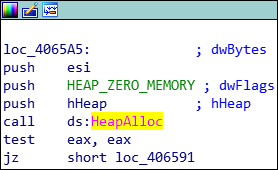
\includegraphics[width=\linewidth]{img/function_call_regular}
            \caption{Regular Windows \gls{api} call}
        \end{subfigure}
        \begin{subfigure}[b]{0.678\textwidth}
            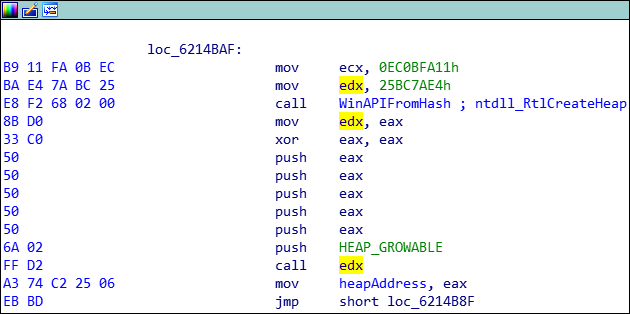
\includegraphics[width=\linewidth]{img/function_call_obfuscated}
            \caption{Obfuscated Windows \gls{api} call}
        \end{subfigure}
    }
    \caption{Windows \gls{api} call obfuscation through \texttt{WinAPIFromHash\label{fig:Windows_API_call_obfuscation}}}
\end{figure}

\autoref{fig:Windows_API_call_obfuscation} demonstrates the difference between a regular imported function call and Dridex's \lstinline|WinAPIFromHash|.
In the standard case, IDA is able to identify the arguments pushed to the stack and add their names to the respective instructions as comments.
Furthermore, they are also properly typed as well as renamed to match the function signature which helps immensely in deciphering the function's purpose.
In contrast, the result of the call to \lstinline|WinAPIFromHash| cannot be statically determined which leaves IDA unable to correctly process the function's arguments.

To overcome this obfuscation layer the python script \lstinline|tag_hashes.py| was written. 
It uses the IDA's Python \gls{api} to find immediate values which look like \gls{dll} or function name hashes and performs a lookup in a set of known values.
If a match is found the script adds a comment to the specific instruction in the IDA database while unknown values are printed with their offset in the binary.
This enables the reverse engineer to iteratively resolve single hashes, add them to the script's knowledge base and rerun the script to annotate all occurrences of the newly found function.

Luckily \lstinline|WinAPIFromHash| is highly self contained and does not require any special setup besides the hashes passed in the standard registers for the \lstinline|fastcall| calling convention, \lstinline|ecx| and \lstinline|edx|.
This permits the reverse engineer to jump through the function's cross-references, selectively load the hashes into the registers and call the function to quickly decode hashes.

\begin{figure}
    \centering
    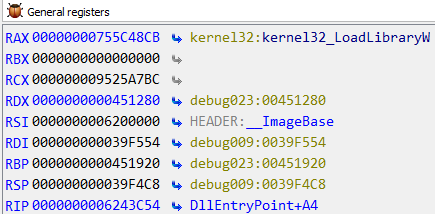
\includegraphics[width=.75\textwidth]{img/memory_annotation_dynamic}
    \caption{Dynamic memory annotations in IDA Pro\label{fig:IDA::Memory_annotation}}
\end{figure}

As shown in \autoref{fig:IDA::Memory_annotation} IDA annotates all uses of named memory locations directly even when they are loaded or calculated dynamically during runtime.
In addition the used notation \lstinline|<binary_without_extension>_<function_name>| can be double clicked to jump to the address if it is currently mapped in the address space.
Therefore, the annotations produced by \lstinline|tag_hashes.py| can be used to quickly navigate to the resolved function if desired.


\section{Summary\label{sec:Reverse_engineering_Dridex::Summary}}
We have now described the Dridex infection process and its most important stages.
The loader uses simple RC4 encryption with an hard-coded key to communicate with the distribution server and is used to download the malicious modules and an initial L2 node \gls{pl}.
The request messages for this process were documented on the byte-level.
Next the modules are injected in multiple processes and executed through an embedded assembly stub.
The execution mechanism inside the stub including its core structure were introduced and detailed in pseudo code.

The main bot module itself is divided into multiple discrete threads which are selected based on the process the module was injected into.
Common targets for injection are browsers which the \gls{mw} is able to hook to extract sensitive information.
We described the roles of each thread with a focus on the one responsible for \gls{bn} communication.
Finally, a comprehensive summary of the \emph{CheckMe} process concludes the chapter.
Next to a conceptual description we also provided message layout figures and detailed important \emph{request types} and \emph{response status codes}.

With the information presented in this chapter we are now prepared to implement the Dridex L2 scanner to verify the correctness of the protocol descriptions.
% !TEX root ../thesis
\chapter{Evaluation\label{ch:Evaluation}}

\abstract{In this chapter we evaluate the results obtained from dissecting Dridex's \gls{p2p} protocol. First the concept and implementation of the \emph{Dridex L2 Scanner} is briefly highlighted. We then motivate the choice of our data sets and present the results obtained by scanning and monitoring them. Finally, the chapter closes with some security considerations of the \gls{p2p} protocol.}

To verify the knowledge obtained from reverse engineering Dridex's \gls{p2p} protocols the \emph{Dridex L2 Scanner} was written.
As the request for \gls{pl} updates could not be completeley documented, real crawling monitoring was not possible.
However, the scanner is able to identify active L2 nodes with high confidence by sending crafted \gls{p2p} protocol messages and parsing the responses.
In addition a small monitoring component was built to track the online status of discovered \glspl{sp}.

\section{Dridex L2 Scanner\label{sec:Evaluation::Dridex_L2_scanner}}
The \emph{Dridex L2 Scanner} was developed to be able to efficiently detect layer 2 nodes in large \gls{ip} address ranges.
To achieve this, we selected the \emph{CheckMe} process (cf:~\autoref{fig:Communication::Bot_stage::Checkme}) from the \gls{p2p} protocol as basis for the scan since the messages are relatively simple, yet provide strong \glspl{ioc}.
The overall process consists of three phases which are depicted in~\autoref{fig:Dridex_L2_scanner::Phases}.
First, in the \emph{pre-selection} phase, a candidate list is built based on open ports in the scanned \gls{ip}-address range.
In the \emph{probing phase} the scanner probes each selected host with a crafted `\lstinline|checkme|' message (cf:~\autoref{bf:P2P::Request::Checkme}) to check for active L2 nodes.
Ultimately, the list of \glspl{ip} which responded with a correct response on the socket are compared with the list of \glspl{ip} which tried to connect to the scan machine on the announced \gls{p2p} port.
Any matches between these two sets indicate an infection at the specific host. \\

\begin{figure}[htb]
    \centering
    \makebox[\linewidth][c]{
        \begin{tikzpicture}[
            node distance = 0mm and 18mm,
            arrowbox/.style = {arrow box,
                arrow box arrows={east:1cm},
                arrow box shaft width=2.5cm,
                arrow box head extend=0mm,
                line width=0,
                text=white,
                font=\sffamily\bfseries,
                inner sep=5mm,
                minimum height=2.5cm,
                minimum width=8em,
                align=center,
                text width=10em,
            }
        ]
            \flowarrowfirst{S3}{\hspace{1.5em}Verification\\\hspace{1.5em}\small{(correlate \glspl{ip})}}{BrickRed}{white}
            \flowarrow{S2}{\hspace{1.5em}Probing\\\hspace{1.5em}\small{(send `\texttt{checkme}')}}{BurntOrange}{white}{S3}
            \flowarrow{S1}{\hspace{1.5em}Pre-selection\\\hspace{1.5em}\small{(based on ports)}}{ForestGreen}{white}{S2}
        \end{tikzpicture}
    }
    \caption{Dridex L2 scanner phases\label{fig:Dridex_L2_scanner::Phases}}
\end{figure}

\begin{description}
    \item[Pre-selection]
    As highlighted in~\autoref{lst:BindPortForP2P} Dridex uses a set of 13 preferred ports for the \gls{p2p} protocol with a fallback mechanism choosing the first free one between \texttt{1000} and \texttt{65000}.
    We use this information to limit our scan to the hosts that have at least one of the preferred ports open as it is highly unlikely that the fallback routine is used on a regular machine that is not a \gls{sandbox}.
    The goal of this phase is to obtain a list of \glspl{ip} listening on at least one of the 13 preferred ports which are later probed.
    For this phase Zmap\fnote{\url{https://zmap.io}} was used as it provides unparalleled scanning speed for large \gls{ip}-address ranges.
    Unfortunately---due to the architecture of the program---only one port can be scanned at once, which resulted in 13 separate runs.
    \item[Probing]
    In this phase the scanner works through the generated \gls{ip} lists from phase 1 in order of port preference and sends a prepared `\texttt{checkme}' request containing a pre-selected port number.
    A Dridex L2 node will obtain the port number from the message, try to initiate a connection and report back the failure on on the same socket the original request was sent.
    The scanner verifies that the response received on the socket is a valid Dridex \gls{p2p} message and records the \gls{ip} addresses of the hosts.
    Any other responses---such as \gls{http} 404/``Not Found'' or \gls{tls} handshake failures---are discarded and ignored.
    The scanning component was implemented in Python as it provides a decent tradeoff between raw performance and the ability to quickly iterate.
    Its \lstinline|socket| functions are almost exclusively direct wrappers around their native C counterparts guaranteeing a high throughput without manual memory management.
    The verification task of the received Dridex responses was separated into a standalone, executable script to make it available for offline analysis.
    \item[Verification]
    While the scan was running a \emph{tcpdump} process captured attempted connections on the advertised \gls{p2p} port for later correlation.
    Although a valid Dridex \gls{p2p} response on the socket is a very strong \gls{ioc}, we compared the \gls{ip} addresses of these hosts with the list of all hosts that initiated a connection on the specified port.
    The combination of these results indicates that either a real Dridex L2 node is running on that host or a sophisticated \gls{sn} by other security researchers (cf:~\autoref{sec:Related_work::Botnets}).
\end{description}

While the Dridex L2 Scanner was built to detect L2 nodes/\glspl{sp} on the public internet, it can also be used inside private networks to identify regular \glspl{bot}.
This is possible because the \gls{mw} always binds and listens on a port even if not instructed by the \gls{c2} as the port is required for the \emph{CheckMe} process to decide if the \gls{bot} could be a \gls{sp}.
This enables the scanner to find the infected machines given that direct routing is possible and traffic is not filtered by a firewall on the network or host.


\section{Data sets\label{sec:Evaluation::Data_sets}}
We verified the scanner on two data sets using knowledge from the first scan to optimize the second run on a larger \gls{ip}-address range.
Key characteristics of both scans are summarized in \autoref{tab:DataSets}.
The first scan was performed on the large subnets\fnote{All subnets containing more than 4096 addresses (``/20'')} allocated to the Great Britain by \acrshort{ripe}.
These networks were chosen specifically because the country was historically the most damaged region by Dridex~\cite{blueliv2015chasing}.
Of course, this does not necessarily mean that many layer 2 nodes are running in these \gls{ip} address ranges but from an administrative standpoint, it makes sense to deploy at least some \glspl{sp} there to guarantee low latencies for data exfiltration.
This scan included 106,033,152 \gls{ip} addresses which attribute for about 2.5\% of the entire \gls{ip4} address space.
1,676,202 of the scanned \gls{ip} addresses were actually probed with the prepared `\lstinline|checkme|' message, because they listened on one or more of the 13 preferred ports.

\begin{table}
    \centering
    \begin{tabular}{rrr}
        \toprule
        &
        \#1: GB subnets > \texttt{/20} &
        \#2: \gls{ripe} \\
        \midrule
        Total \gls{ip}s &
        106,033,152 (02.47\%)\(^\dag\) &
        814,461,240 (18.96\%)\(^\dag\)\\

        Probed unique \gls{ip}s &
        1,676,202 (00.04\%)\(^\dag\) &
        11,040,833 (00.26\%)\(^\dag\)\\

        Scanned ports &
        all 13 &
        top 4\\

        Bytes send &
        \({\sim}\)3600 MB\(^\ddag\) &
        \({\sim}\)8600 MB\\

        Scan time &
        35:00 hours &
        20:35 hours\\
        \bottomrule
        \multicolumn{3}{l}{\(^\dag\) percentage of the \gls{ip4}-address space} \\
        \multicolumn{3}{l}{\(^\ddag\) estimated value} \\
    \end{tabular}
    \caption{Verification data sets for Dridex L2 Scanner\label{tab:DataSets}}
\end{table}

For the second scan we extended the \gls{ip}-address range to cover all addresses assigned by \gls{ripe} totaling in 814,461,240 \gls{ip}s.
The results obtained from this first data set prompted us to limit this scan to the first four preferred ports (cf:~\autoref{lst:BindPortForP2P}).
Given that Dridex is most prevalent in Europe and with about 19\% of the \gls{ip4} address space scanned, this data set may hint at Dridex's population count.
This run finished significantly faster as the scanner was optimized to open 1024 concurrent connections instead of the previous 256.

\begin{quote}
\textbf{Remark:} The \gls{ip}-address ranges for both data sets were obtained from an official list by \gls{ripe} retrieved from \url{ftp://ftp.ripe.net/pub/stats/ripencc/delegated-ripencc-extended-latest} on the 02.11.2017.
Country allocation was determined solely by the identifier in the second column.
\end{quote}


\section{Results\label{sec:Evaluation::Results}}
After scanning the first data set we received three distinct responses that the scanner categorized as valid Dridex responses.

\begin{description}
    \item[Dridex]
    This category of messages heavily suggests either a Dridex L2 node or a sensor node running on the probed host as the response matched the expected behavior exactly.
    The message returned contained the expected status code ``0404'' which indicates a failed \emph{CheckMe} process.
    As the scanner does not listen on the port specified in the request the node cannot connect to it and returns the error appropriately.
    All of these hosts could also be found when matching the \gls{ip} addresses of these host with the attempted connections on the advertised port.
    Each host tried to establish a connection exactly three times directly after receiving the `\lstinline|checkme|' request further hinting at protocol conform behavior.
    \item[Empty]
    In the first run the scanner marked some \glspl{ip} with an empty response inside the \gls{p2p} envelope (cf:~\autoref{bf:P2P::Envelope}), which was unexpected according to the analyzed Dridex sample.
    At first glance this could point at either poorly implemented \glspl{sn} or perhaps Dridex L2 nodes running a newer version with a changed response format for the `\lstinline|checkme|' request.
    Unfortunately, the scanner hat a bug in parsing responses during the scan of the first data set.
    Responses with a length of exactly 168 bytes were reported as valid but not to have any payload.
    Most probably, all responses in this category come from applications other than Dridex and were wrongly classified because of this bug.
    This is supported by the fact, that we did not observe any more messages of this category during the scan of the second data set with a fixed version of the scanner.
    \item[Echo]
    Several hosts implemented a concept commonly referred to as \emph{Echo Server}.
    Each incoming message is directly sent back to the sender, effectively mirroring the request.
    Because the scanner only detects and unwraps the \gls{p2p} message envelope, the crafted `\lstinline|checkme|' message was classified as valid.
    Although not particularly interesting in itself the hosts did technically send valid Dridex messages which could be monitored by netflow analysis in transit.
\end{description}

\begin{figure}
    \centering
    \begin{tikzpicture}
        \begin{axis}[
            xbar stacked,
            ytick=data,
            nodes near coords,
            symbolic y coords={8000,8080,80,3443,8443,443},
            xlabel={Amount of received messages},
            ylabel={Port number},
            enlarge x limits=0,
            xmax=45,
            legend cell align=left,
            height=8cm,
            width=.8\linewidth,
            bar width=20pt]
            \addplot[draw=red!50!black, fill=red!50] coordinates
                {(21,443) (1,8443) (1,3443) (0,80) (0,8080) (0,8000)};
            \addplot[draw=blue!50!black, fill=blue!50] coordinates
                {(2,443) (1,8443) (0,3443) (9,80) (2,8080) (1,8000)};
            \addplot[draw=gray!30!black, fill=gray!50] coordinates
                {(2,443) (0,8443) (0,3443) (34,80) (4,8080) (1,8000)};
            \legend{Dridex, Empty, Echo};
        \end{axis}
    \end{tikzpicture}
    \caption{Dridex L2 Scanner results for data set \#1\label{fig:ScanResults::GB}}
\end{figure}

The results of scanning the first data set are shown in \autoref{fig:ScanResults::GB}.
The majority of the potential Dridex L2 nodes are handling the \gls{p2p} protocol on the port 443 with few exceptions using 8443 and 3443.
This is consistent with the local tests on the analyzed main bot module sample, which would always pick the first free port from the hard-coded list of preferred ports (cf:~\autoref{lst:BindPortForP2P}).
Based on these results all future scans were reduced to only probe the first four ports in the list (443, 8443, 3443, 4443) as it seems highly unlikely that the \gls{mw} would choose a port beyond that.
This is especially true as the ports 3443 and 4443 are assigned to rarely used programs according to \gls{iana}'s database.
It might make sense to consistently scan all preferred ports to detect peers purposefully listening on exotic ports which might be \glspl{sn} or maybe even \glspl{hp} operated by the Dridex \glspl{bm}.
However, even for these use-cases, it seems more efficient to just use a standard port to attract more traffic.

With the results obtained from the first data set the scanner was optimized to directly identify echo servers and discard the wrongly classified empty messages.
The scan of the second data set, the entire address space manageged by \gls{ripe}, revealed more L2 nodes.
After the scan the total L2 node count was 42, only 19 more than the initial 23 found in Great Britain.
This value is especially confusing as some nodes originally found in the first scan were not present anymore in the second scan.
To measure the distribution across the different countries, a \lstinline|whois| query was issued for each \gls{ip} address and filtered by the ``[Cc]ountry'' field.
The absolute results can be found in \autoref{tab:ScanResults::RIPE::Country}, while \autoref{fig:ScanResults:RIPE::Country} shows the percentages.
Interestingly the scan found 10 additional L2 nodes in Great Britain for a total of 33 (or 78.57\% of all infections).
Although we expected a higher percentage due to Dridex's targeting of this area, this value seems comparatively high.
The results of other countries are roughly as expected from the percentage of \gls{ip} addresses with only Ireland beeing slightly overrepresented.

\begin{figure}
    \begin{floatrow}
        \capbtabbox{%
        \begin{tabular}{lrr}
            \toprule
            Country &
            \# \glspl{ip} &
            \# L2 nodes\\
            \midrule
            GB &
            122,734,616 &
            33\\

            FR &
            80,898,864 &
            2\\

            IT &
            53,982,016 &
            1\\

            SE &
            30,079,336 &
            2\\

            NO &
            15,858,064 &
            1\\

            IE &
            6,493,776 &
            2\\

            BG &
            4,440,064 &
            1\\

            \textsc{Rest} &
            499,974,504 &
            0 \\
            \midrule
            \textsc{Total} &
            814,461,240 &
            42\\
            \bottomrule
        \end{tabular}\vspace{.75em}}{\caption{\gls{ripe}: \gls{ip} and L2 node counts per country\label{tab:ScanResults::RIPE::Country}}}
        \ffigbox{%
        \begin{tikzpicture}
            \begin{axis}[
                ybar,
                xtick=data,
                nodes near coords,
                every node near coord/.append style={rotate=90, anchor=west},
                symbolic x coords={GB,FR,IT,SE,NO,IE,BG},
                ylabel={Percentage},
                enlarge y limits={upper,value=0.275},
                legend cell align=left,
                height=7cm,
                bar width=10pt]
                \addplot [draw=blue!50!black, fill=blue!50] coordinates {
                    (GB,15.069423807080125753)
                    (FR,9.932807115535663797)
                    (IT,6.627941680809758362)
                    (SE,3.693157454613800897)
                    (NO,1.947061839308645308)
                    (IE,0.797309396822861699)
                    (BG,0.545153505401926800)
                };
                \addplot [draw=red!50!black, fill=red!50] coordinates {
                    (GB,78.571428571428571429)
                    (FR,4.761904761904761905)
                    (IT,2.380952380952380952)
                    (SE,4.761904761904761905)
                    (NO,2.380952380952380952)
                    (IE,4.761904761904761905)
                    (BG,2.380952380952380952)
                };
                \legend{Allocated \glspl{ip}, Dridex L2 nodes};
            \end{axis}
        \end{tikzpicture}}{\caption{\gls{ripe}: \gls{ip} and L2 node percentages per country\label{fig:ScanResults:RIPE::Country}}}
    \end{floatrow}
\end{figure}

There are two possible explanations for the unexpected distribution of L2 nodes in Great Britain and the low total number of \glspl{sp} in the \gls{ripe} subnets.
On the one hand, the total number of \gls{ip} addresses per country is calculated by summing up the subnet numbers given in the original file from \gls{ripe} while the country allocation of the infected hosts was determined via \lstinline|whois|.
This could lead to differences, e.g., in cases where an \gls{ip} address is allocated to another country which then resells it to a company or private customer in Great Britain, resulting in a changed \lstinline|whois| entry.
On the other hand, we later discovered that the maximum socket count in the probing phase for the \gls{ripe} data set was set too high which might have resulted in packet drops, possibly missing positive response messages.
Due to time constraints the scan could not be repeated in time but the obtained results should provide a general indication of Dridex's presence in Europe.

\begin{figure}
    \centering
    \begin{tikzpicture}
        \begin{axis}[
            % Type
            %only marks,
            % Setup
            table/col sep=comma,
            date coordinates in=x,
            date ZERO=2017-11-12,
            % Labels
            xlabel={Time of day},
            xticklabel={\hour:\minute},
            xticklabel style={rotate=30, anchor=near xticklabel},
            enlarge x limits=.025,
            ylabel={\# of online L2 nodes},
            xtick distance={0.125},
            ytick distance=2,
            legend pos=north west,
            legend cell align=left,
            % Misc
            width=15cm]
            \addplot+[mark=x, draw=gray, line width=1.25pt] table[x=ts,y=avg] {data/crawler.csv};
            \addplot+[mark=x, draw=blue!50] table[x=ts,y=min] {data/crawler.csv};
            \addplot+[mark=x, draw=red!70] table[x=ts,y=max] {data/crawler.csv};
            \addplot+[mark=none, draw=gray!50, line width=1pt, dashed] table[x=ts,y=total_avg] {data/crawler.csv};
            \legend{Average, Min, Max, Total average}
        \end{axis}
    \end{tikzpicture}
    \caption{Active L2 nodes during the day between 12.--15.11.2017\label{fig:CrawlingResults}}
\end{figure}

To gain more insights about the uptime of the detected L2 nodes, the probing component was adapted to use a newly crafted `\lstinline|ping|' request message (cf:~\autoref{bf:P2P::Request::Ping}).
This request type was chosen over the previously used `\lstinline|checkme|' as it does not prompt the L2 node to initiate a connection improving the response time.
Additionally, the `\lstinline|pong|' response contains the node's BotId delivering even more data to analyze.
\autoref{fig:CrawlingResults} shows the results obtained from checking the online status of the known bots between 12.11.2017--15.11.2017.
The x-axis shows the time of day from 00:00 to 24:00; the plot illustrates the average, minimum and maximum number of active L2 nodes measured for any given 15 minutes among all four days.
From the 42 unique \glspl{ip} found only a total of 24 were online at peak times during the monitoring process.
This can be attributed to \gls{node_churn} or non-static \gls{ip} addresses (very common in non-professional connection setups).
As the request for \gls{pl} updates could not be reverse engineered this remains a problem in the current monitoring approach.

Although the monitoring window was very short, a trend is visible showing more active \glspl{sp} during typical work hours and slightly past that.
Especially visible is the sharp rise at 09:00 passing the total average of 16 active \glspl{sp} and the steady decline starting at around 16:00.
This seems to indicate that at least some of the crawled L2 nodes are running on office computers which get shut down later in the day.
However, longer crawling timespans and a larger set of known \glspl{ip} are definitely required to verify this claim.

Another interesting fact was revealed when BotIds were crawled for all known infected hosts.
A set of 5 closely related \gls{ip} addresses (in the same ``/29'' subnet) all returned the exact same BotId: \lstinline|OFFICE_4ecea422c76a2a58da6e42c7c47f283c|.
The clash heavily implies either a cloned \gls{vm} instance, a machine that is available from multiple \gls{ip} addresses or a simple \gls{sn}/\gls{hp} implementation with a hard-coded setting for this property because this value is computed from unique values of the Windows registry 
As a \lstinline|whois| query did not immediately reveal a particular research or commercial entity behind the hosts, this theory could not be confidently verified.

    %IE 6493776
    %PL 20868168
    %BE 28447104
    %SE 30079336
    %ES 30521664
    %RU 45087744
    %NL 47058400
    %IT 53982016
    %FR 80898864
    %DE 120098432
    %GB 122734616

    % 814461240

    % 33 GB
    %  2 FR
    %  2 IE
    %  2 SE
    %  1 IT
    %  1 BG
    %  1 no

\section{Security considerations\label{sec:Evaluation::Security_considerations}}
When analyzing the communication protocols and especially the \gls{p2p} protocol we found two minor weaknesses that might be useful in monitoring and takedown attempts.
While none of them is trivially exploitable they still present significant opportunities for possible takedown attempts.

\begin{description}
    \item[Missing buffer length validation]
    In several places the functions responsible for protocol handling use length values directly read from a message without verifying that the message buffer actually contains the requested amount of data.
    While the envelope handling is quite robust---discarding all invalid messages reliably---the actual message handling often relies valid messages.
    One example is the encrypted BotId that is mandatory in every \gls{p2p} request (cf:~\autoref{bf:P2P::Request}).
    If the encoded string is omitted the following message content is directly interpreted as a length argument leading to an \emph{access violation} terminating the execution.
    This is not as critical as one might imagine as each incoming connection gets handled in a newly spawned thread, but it nonetheless demonstrates that the binary contains possibly exploitable vulnerabilities.
    \item[Protocol inconsistency]
    As mentioned above the `\lstinline|ping|' message was used to continuously crawl the known L2 nodes.
    This message is only used to check whether a new \gls{bot} can be promoted to a \gls{sp}.
    Since the L2 nodes are already \glspl{sp} they should not even be required to handle this request type unless it is also used for some kind of \gls{c2} heartbeat.
    Unfortunately the analysis did not cover the \gls{c2} protocol but it seems unlikely that a layer 3 node (or even the \gls{c2}) would use a request from the \gls{p2p} protocol for such a purpose.
    Until this inconsistency is addressed, the `\lstinline|ping|' request remains a good way to cheaply detect the online status of L2 nodes and retrieve their BotId which is also included in the `\lstinline|pong|' response.
\end{description}


\section{Summary\label{sec:Evaluation::Summary}}
The Dridex L2 scanner is able to reveal active L2 nodes in large \gls{ip}-address spaces in reasonable time.
With the detection of 42 \glspl{sp} throughout the European \gls{ip}-address space we have strong indications that the protocol descriptions presented earlier are accurate for the sample that we analyzed.

As only one sample of the main bot module was dissected it cannot be verified that this protocol is generally used by all Dridex subnets.
However, the presence of active L2 nodes in multiple countries---8 month after the sample was discovered in the wild---suggest that multiple subnets still use the exact protocol today.
Additionally, the set of L2 nodes was monitored for a short amount of time, revealing a pattern in their uptime which indicates that some of them are running in office environments.
This assumption could be further verified by extended monitoring across a larger timeframe.
% !TEX root ../thesis
\chapter{Conclusion\label{ch:Conclusion}}

This thesis analyzed the Dridex \gls{bn} and presented descriptions of its architecture and communication protocols.
With the knowledge acquired we were able to detect and monitor a limited set of \glspl{sp}/layer 2 (L2) nodes which indicates that these host actually communicate through the protocols discovered.


\section{Results}\label{sec:Conclusion::Results}
From an architectural standpoint we covered the whole infection process starting from the dropper up to the complete \gls{bot} stage.
Every component was described as accurately as possible with an extended focus on the main bot module as it is responsible for the communication with the \gls{bn} and \gls{c2}.
We briefly documented the several functionalities provided by the module as well as a selection of obfuscation techniques that were encountered.
The focus was placed on byte-exact representations of all network communication to bootstrap further research.

To efficiently detect L2 nodes in large \gls{ip}-address ranges we chose to emulate the \emph{CheckMe} process.
This part of the \gls{p2p} protocol forces the \gls{sp} to attempt a connection to the scanning host.
Correlating the \gls{ip} addresses that returned a proper, protocol conforming message with the hosts that tried to establish a connection during the scan provides a strong \gls{ioc}.
For the monitoring component the `\lstinline|ping|' request was chosen as it increases response time allowing for quicker uptime probing.

As Great Britain was a major target of past Dridex campaigns, we performed a scan of all large subnets allocated to this region.
Although the analyzed sample, and therefore the campaign, was released 8 month ago, we were able to verify 42 total \glspl{sp} across Europe.
We monitored the detected L2 nodes, building up an uptime profile throughout the day and retrieving their unique \emph{BotId}.
The results obtained supported the theory that a subset of \gls{sp} are running on office machines which are turned off in the evening.
Finally, a potential vulnerability and an information leak were discovered which might aid in future takedown attempts.


\section{Future work}\label{sec:Conclusion::Future_work}
While this thesis provides a solid basis for understanding and monitoring the malware, several aspects should be covered in more detail in future work.
Based off the knowledge presented, certain questions remain open.

\begin{description}
    \item[Continuous monitoring]
    Although the scanning and crawling were highly important to verify the basic understanding of the \gls{p2p} communication, the gathered data remains inconclusive for real assumptions about Dridex's size and reach.
    To gain further insights into the \gls{bn}'s population counts, longer, continuous monitoring is essential.
    This would also help to detect changes and updates in the protocol as it has already evolved several times in the past.
    \item[Binary and \gls{pl} updates]
    The mechanisms and protocol messages for both binary and \gls{pl} updates were out of scope for this thesis and propose a promising research question.
    As these processes change the state on the infected host, they could contain a vulnerability to potentially take down Dridex.
    Additionally these requests are essential for a traditional crawling approach to deal with \gls{node_churn} without having to rescan the whole Internet periodically.
    \item[Prevention]
    Details about the loader stage and especially the memory injection technique and target processes were not fully analyzed in this thesis as they do not directly influence communication protocols.
    This limits the results' usefulness in prevention scenarios particularly on end-user machines which (usually) cannot be scanned from the open Internet.
    Future research could help identify Dridex during the infection process for example through registry keys or the initial \gls{pl} download from the distribution server.
    \item[Vulnerabilty analysis]
    While we discovered a weakness in length validations in several functions handling the \gls{p2p} protocol, it remains unclear, if these can be exploited in a meaningful way to manipulate or cleanup a Dridex infection.
    In combination with the research about the update process mentioned above, this could assist in a future takedown attempt.
\end{description}

% Bibliography
\printbibliography%

% Lists of *
\microtypesetup{protrusion=false} % disable protrusion locally for the following lists

% We don't want new pages after these "chapters"
\begingroup
%\renewcommand{\cleardoublepage}{}
%\renewcommand{\clearpage}{}
\let\cleardoublepage\clearpage

\listoffigures
\listoftables
\lstlistoflistings%

\endgroup

\microtypesetup{protrusion=true}  % reenable protrusion

% Appendices
\begin{appendices}
% !TEX root ../thesis
% /* spellchecker: disable */
\printglossary[type=\acronymtype]
\printglossary

\chapter{Hashes}\label{ap:Hashes}

\begin{table}[H]
    \centering
    \makebox[\linewidth][c]{
        \begin{tabular}{rl}
            \toprule
            Component &
            MD5\\
            \midrule

            Dridex loader &
            \texttt{760390f07cefafadece0638a643d69964433041abeab09b65bfcdb922c047872}\\

            Bot main module &
            \texttt{166bd27de260cccbfcdcb21efc046288043bd44c4f08e92cd1e1f9eb80cca7ff}\\
        \end{tabular}
    }
    \caption{Hashes of analyzed samples\label{tab:Hashes}}
\end{table}

\begingroup
\renewcommand{\cleardoublepage}{}
\renewcommand{\clearpage}{}
\chapter{Source code}\label{ap:Source_code}
\endgroup

\lstinputlisting[caption={DridexWinApiNames}, label={lst:Types::DridexWinApiNames},style=c]{code/dridex_win_api_names.h}

\lstinputlisting[caption={DridexInitStruct (full)}, label={lst:Types::DridexInitStruct_full},style=c]{code/dridex_init_struct.h}

\end{appendices}

\newpage

\thispagestyle{empty}

\chapter*{}

% Eidesstattliche Erklärung
\section*{Eidesstattliche Erklärung}

Hiermit versichere ich an Eides statt, dass ich die vorliegende Arbeit im Master-
studiengang Informatik selbstständig verfasst und keine anderen als die angegebe-
nen Hilfsmittel---insbesondere keine im Quellenverzeichnis nicht benannten Internet-
Quellen---benutzt habe. Alle Stellen, die wörtlich oder sinngemäß aus Veröffentlichun-
gen entnommen wurden, sind als solche kenntlich gemacht. Ich versichere weiterhin,
dass ich die Arbeit vorher nicht in einem anderen Prüfungsverfahren eingereicht habe
und die eingereichte schriftliche Fassung der auf dem elektronischen Speichermedium
entspricht.

\bigskip
\bigskip

Hamburg, den \leadingzero{\day}.\leadingzero{\month}.\leadingzero{\year} \quad \dotfill

\end{document}
